% Template for PLoS
% Version 3.4 January 2017
%
% % % % % % % % % % % % % % % % % % % % % %
%
% -- IMPORTANT NOTE
%
% This template contains comments intended 
% to minimize problems and delays during our production 
% process. Please follow the template instructions
% whenever possible.
%
% % % % % % % % % % % % % % % % % % % % % % % 
%
% Once your paper is accepted for publication, 
% PLEASE REMOVE ALL TRACKED CHANGES in this file 
% and leave only the final text of your manuscript. 
% PLOS recommends the use of latexdiff to track changes during review, as this will help to maintain a clean tex file.
% Visit https://www.ctan.org/pkg/latexdiff?lang=en for info or contact us at latex@plos.org.
%
%
% There are no restrictions on package use within the LaTeX files except that 
% no packages listed in the template may be deleted.
%
% Please do not include colors or graphics in the text.
%
% The manuscript LaTeX source should be contained within a single file (do not use \input, \externaldocument, or similar commands).
%
% % % % % % % % % % % % % % % % % % % % % % %
%
% -- FIGURES AND TABLES
%
% Please include tables/figure captions directly after the paragraph where they are first cited in the text.
%
% DO NOT INCLUDE GRAPHICS IN YOUR MANUSCRIPT
% - Figures should be uploaded separately from your manuscript file. 
% - Figures generated using LaTeX should be extracted and removed from the PDF before submission. 
% - Figures containing multiple panels/subfigures must be combined into one image file before submission.
% For figure citations, please use "Fig" instead of "Figure".
% See http://journals.plos.org/plosone/s/figures for PLOS figure guidelines.
%
% Tables should be cell-based and may not contain:
% - spacing/line breaks within cells to alter layout or alignment
% - do not nest tabular environments (no tabular environments within tabular environments)
% - no graphics or colored text (cell background color/shading OK)
% See http://journals.plos.org/plosone/s/tables for table guidelines.
%
% For tables that exceed the width of the text column, use the adjustwidth environment as illustrated in the example table in text below.
%
% % % % % % % % % % % % % % % % % % % % % % % %
%
% -- EQUATIONS, MATH SYMBOLS, SUBSCRIPTS, AND SUPERSCRIPTS
%
% IMPORTANT
% Below are a few tips to help format your equations and other special characters according to our specifications. For more tips to help reduce the possibility of formatting errors during conversion, please see our LaTeX guidelines at http://journals.plos.org/plosone/s/latex
%
% For inline equations, please be sure to include all portions of an equation in the math environment.  For example, x$^2$ is incorrect; this should be formatted as $x^2$ (or $\mathrm{x}^2$ if the romanized font is desired).
%
% Do not include text that is not math in the math environment. For example, CO2 should be written as CO\textsubscript{2} instead of CO$_2$.
%
% Please add line breaks to long display equations when possible in order to fit size of the column. 
%
% For inline equations, please do not include punctuation (commas, etc) within the math environment unless this is part of the equation.
%
% When adding superscript or subscripts outside of brackets/braces, please group using {}.  For example, change "[U(D,E,\gamma)]^2" to "{[U(D,E,\gamma)]}^2". 
%
% Do not use \cal for caligraphic font.  Instead, use \mathcal{}
%
% % % % % % % % % % % % % % % % % % % % % % % % 
%
% Please contact latex@plos.org with any questions.
%
% % % % % % % % % % % % % % % % % % % % % % % %

\documentclass[10pt,letterpaper]{article}
\usepackage[top=0.85in,left=2.75in,footskip=0.75in]{geometry}

% amsmath and amssymb packages, useful for mathematical formulas and symbols
\usepackage{amsmath,amssymb}

% Use adjustwidth environment to exceed column width (see example table in text)
\usepackage{changepage}

% Use Unicode characters when possible
\usepackage[utf8x]{inputenc}

% textcomp package and marvosym package for additional characters
\usepackage{textcomp,marvosym}

% cite package, to clean up citations in the main text. Do not remove.
\usepackage{cite}

% Use nameref to cite supporting information files (see Supporting Information section for more info)
\usepackage{nameref,hyperref}

% line numbers
\usepackage[right]{lineno}

% ligatures disabled
\usepackage{microtype}
\DisableLigatures[f]{encoding = *, family = * }

% color can be used to apply background shading to table cells only
\usepackage[table]{xcolor}

% array package and thick rules for tables
\usepackage{array}

% create "+" rule type for thick vertical lines
\newcolumntype{+}{!{\vrule width 2pt}}

% create \thickcline for thick horizontal lines of variable length
\newlength\savedwidth
\newcommand\thickcline[1]{%
  \noalign{\global\savedwidth\arrayrulewidth\global\arrayrulewidth 2pt}%
  \cline{#1}%
  \noalign{\vskip\arrayrulewidth}%
  \noalign{\global\arrayrulewidth\savedwidth}%
}

% \thickhline command for thick horizontal lines that span the table
\newcommand\thickhline{\noalign{\global\savedwidth\arrayrulewidth\global\arrayrulewidth 2pt}%
\hline
\noalign{\global\arrayrulewidth\savedwidth}}


% Remove comment for double spacing
%\usepackage{setspace} 
%\doublespacing

% Text layout
\raggedright
\setlength{\parindent}{0.5cm}
\textwidth 5.25in 
\textheight 8.75in

% Bold the 'Figure #' in the caption and separate it from the title/caption with a period
% Captions will be left justified
\usepackage[aboveskip=1pt,labelfont=bf,labelsep=period,justification=raggedright,singlelinecheck=off]{caption}
\renewcommand{\figurename}{Fig}

% Use the PLoS provided BiBTeX style
\bibliographystyle{plos2015}

% Remove brackets from numbering in List of References
\makeatletter
\renewcommand{\@biblabel}[1]{\quad#1.}
\makeatother

% Leave date blank
\date{}

% Header and Footer with logo
\usepackage{lastpage,fancyhdr,graphicx}
\usepackage{epstopdf}
\pagestyle{myheadings}
\pagestyle{fancy}
\fancyhf{}
\setlength{\headheight}{27.023pt}
\lhead{\includegraphics[width=2.0in]{PLOS-submission.eps}}
\rfoot{\thepage/\pageref{LastPage}}
\renewcommand{\footrule}{\hrule height 2pt \vspace{2mm}}
\fancyheadoffset[L]{2.25in}
\fancyfootoffset[L]{2.25in}
\lfoot{\sf PLOS}

%% Include all macros below

\newcommand{\lorem}{{\bf LOREM}}
\newcommand{\ipsum}{{\bf IPSUM}}

%% END MACROS SECTION


\begin{document}
\vspace*{0.2in}

% Title must be 250 characters or less.
\begin{flushleft}
{\Large
\textbf\newline{The `Paris-end' of town? Urban typology through machine learning.} % Please use "sentence case" for title and headings (capitalize only the first word in a title (or heading), the first word in a subtitle (or subheading), and any proper nouns).
}
\newline
% Insert author names, affiliations and corresponding author email (do not include titles, positions, or degrees).
\\
Kerry A. Nice\textsuperscript{1*},
Jason Thompson\textsuperscript{1},
Jasper S. Wijnands\textsuperscript{1},
Gideon D.P.A. Aschwanden\textsuperscript{1},
Mark Stevenson\textsuperscript{1},
\\
\bigskip
\textbf{1} Transport, Health, and Urban Design Hub, Faculty of Architecture, Building, and Planning, University of Melbourne, Victoria 3010, Australia
\\
\bigskip

% Insert additional author notes using the symbols described below. Insert symbol callouts after author names as necessary.
% 
% Remove or comment out the author notes below if they aren't used.
%
% Primary Equal Contribution Note
%\Yinyang These authors contributed equally to this work.

% Additional Equal Contribution Note
% Also use this double-dagger symbol for special authorship notes, such as senior authorship.
%\ddag These authors also contributed equally to this work.

% Current address notes
%\textcurrency Current Address: Dept/Program/Center, Institution Name, City, State, Country % change symbol to "\textcurrency a" if more than one current address note
% \textcurrency b Insert second current address 
% \textcurrency c Insert third current address

% Deceased author note
%\dag Deceased

% Group/Consortium Author Note
%\textpilcrow Membership list can be found in the Acknowledgments section.

% Use the asterisk to denote corresponding authorship and provide email address in note below.
* kerry.nice@unimelb.edu.au

\end{flushleft}
% Please keep the abstract below 300 words
\section*{Abstract}
The confluence of recent advances in availability of geospatial information, computing power, and artificial intelligence offers new opportunities to understand how and where our cities differ and also, how they are alike. Departing from a traditional `top-down' analysis of urban design features, this project analyses millions of images of urban form (consisting of street view, satellite imagery, and street maps). A (novel) neural network-based framework is trained with imagery from the largest 1692 cities in the world and the resulting trained models are used to compare within-city locations from Melbourne and Sydney to determine the closest connections between these areas and their international comparators. This work demonstrates a new, consistent, and objective method for understanding the relationship between cities around the world, and the health, transport, and environmental consequences of their design. The results show specific advantages and disadvantages using each type of imagery, and we draw some conclusions about the best use of each for specific analytic goals. Finally, and perhaps most importantly, this research also answers the age-old question, ``Is there really a `Paris-end' of your city?''.

%\keywords{machine learning, urban typology, urban design, transport, health}

% Please keep the Author Summary between 150 and 200 words
% Use first person. PLOS ONE authors please skip this step. 
% Author Summary not valid for PLOS ONE submissions.   
\section*{Author summary}
TODO 

We ask that all authors of research articles include a 150–200 word non-technical summary of the work as part of the manuscript to immediately follow the abstract. This text is subject to editorial change, should be written in the first-person voice, and should be distinct from the scientific abstract.

Aim to highlight where your work fits within a broader context; present the significance or possible implications of your work simply and objectively; and avoid the use of acronyms and complex terminology wherever possible. The goal is to make your findings accessible to a wide audience that includes both scientists and non-scientists.

Authors may benefit from consulting with a science writer or press officer to ensure they effectively communicate their findings to a general audience.
Example Author Summaries
 

Systems Analysis of Chaperone Networks in the Malarial Parasite Plasmodium falciparum

Protein–Protein Interaction Hotspots Carved into Sequences

Elucidating the Altered Transcriptional Programs in Breast Cancer using Independent Component Analysis

\linenumbers



\section*{Introduction}\label{sec:introduction}


Cities are now home to the majority of the world's population with trends predicting continued growth in urbanisation \cite{UNDESA2015,WHO2016}. Residents in the 2015 United Nations list of cities with populations exceeding 300,000 residents \cite{UN2014} account for 2.2 billion people (or approximately 31\% of the world's population) in 2015. Australia, in particular, leads this trend of high urbanisation. In 2013, 65\% of Australians lived in capital cities and it is estimated that this will increase to 72\% by 2053  \cite{ABS2008}. These projections are reflected in population growth estimates that will see the country's population likely increase from 24 million today to over 33 million by 2050 \cite{ABS2008}. This growth is expected to mostly take place within the four largest capital cities (Sydney, Melbourne, Brisbane, and Perth) with projections indicating that by 2053 both Sydney and Melbourne will have populations of almost 8 million  \cite{CommonwealthofAustralia2010}. As a consequence of this population growth in urban areas, an array of planning, transportation, and population health challenges will emerge.

The importance of integrating transport plans with decisions regarding land-use is being recognised by governments \cite{ATAP2016,SAustralia2015}. Land-use decisions significantly influence transport options and travel choice. Further, the high levels of low-density suburbanisation and high car dependency that characterise many cities (in Australia, New Zealand, the United States, and more) are remnants of a mid-twentieth century focus on home and car ownership \cite{Currie2007,Dodson2008}. As a consequence, the status and practical utility of cycling or walking for daily travel requirements is limited \cite{Heesch2014,Daley2011}. Low-density housing renders the cost of large-scale public transport prohibitive, producing a reliance on private vehicles and increasing exposure to risks associated with traffic speed, volume, emissions, and physical inactivity  \cite{Cepeda2016,MingWen2008,Norman2006}. Although some progress has been made in promoting active modes of transport the percentage of Australians walking or cycling to work remains low and primarily concentrated in low-speed, inner-city areas where distances are minimal. Public health policy-makers and urban/transport planners have an opportunity to change this situation by embracing strategies that proactively support active transport modes as facilitated by urban designs witnessed in other countries around the world.

For example, Copenhagen's significant long-term investment in cycling infrastructure, over 2 billion DKK (\texteuro 268 million) since 2004 \cite{Copenhagen2017b} for a city of approximately 550,000 residents, has seen its rates of cycling mode share expand to 45\% of all trips without consequent increases in road trauma \cite{Kaplan2014}. Similarly, Amsterdam's (and the Netherlands more generally) continued leadership in active transport promotion has demonstrated that cycling and walking can be re-claimed in areas and streets previously lost to car traffic, producing both health and economic benefit \cite{Andersen2000}. Substantial published evidence indicates that land-use affects transport modal choice and behaviour  \cite{Giles-corti2016,Kleinert2016,Goenka2016}. In addition, improved population health outcomes related to chronic conditions such as respiratory disease, cardiovascular disease, and Type 2 diabetes are strongly linked with more active transport modal choices  \cite{Zapata-Diomedi2017}. Therefore, the creation of cities and precincts that facilitate greater uptake of safe, active transport could produce manifold environmental, productivity, and population health benefits. 

However, understanding the association between urban design features, transport networks, and health or environmental outcomes remains difficult, especially when underlying data, locations, methods, and demographics upon which statistical models are built vary considerably. As a result, globally consistent comparisons between cities are difficult to achieve. To overcome these limitations, we develop a new framework using an entirely new and highly efficient `bottom-up` approach. Utilising recent advances in computing power and artificial intelligence, as well as an increased availability of globally consistent urban imagery, we train three neural networks with using millions of images of urban form (consisting of street view, satellite imagery, and street maps) from hundreds of world-wide cities. 

Paris, France is a widely recognizable international iconic city \cite{Anholt2006}, leading to many cities to claim that they have a `Paris-end' of town \cite{Williams2010}, or are a Paris on the [insert name of local river] \cite{Wilden2013} (i.e. Paris on the Yarra). Melbourne and Sydney are no exception to this rule. Visual elements of Paris are widely recognizable \cite{Doersch2012}, but can Melbourne or Sydney truly claim to have a `Paris-end'? Is Melbourne `Paris on the Yarra' or Sydney `Paris on the Parramatta'? Using the trained neural networks, we evaluate a systematic sampling of imagery from Melbourne and Sydney to find the closest connections between these areas and their international comparators, testing whether either Melbourne or Sydney can really claim to be `Paris-like'.

However, while potentially making some local tourist boards unhappy (the results definitively answer the question with a `no', `no', and `no' for both cities using three data sets), we also present a fundamental methodology to objectively analyse urban areas using big data imagery. In the process of answering this question, we uncover some specific advantages and disadvantages to analysis using each different type of imagery. We find that each of these data sources uncovers a unique set of urban typology characteristics and that successfully using this analysis technique for urban typological purposes requires an understanding of what characteristics will be emphasised by the varying training data sets.




\section*{Methods}\label{sec:methods}
\subsection*{Neural network}\label{sec:methods1}

The methods in this study are based on artificial intelligence, in particular deep neural networks \cite{Bishop1995,Samarasinghe2016,Graupe2013}. Neural network architectures that have proven to be particularly successful at image recognition tasks are convolutional neural networks \cite{Schmidhuber2015}. These networks generally consist of alternating layers with convolution operations (for feature identification) and max-pooling operations (improving translation invariance and reducing dimensionality). To increase robustness of these complex models, techniques such as weight regularisation and dropout can be applied \cite{Srivastava2014}.

The model for image recognition used in this study is based on a newer version of the Inception architecture \cite{Szegedy2015}, which demonstrated better computer vision performance than any other methodology during the ImageNet Large-Scale Visual Recognition Challenge (ILSVRC) \cite{Russakovsky2015} in 2014. In particular, we use the third version of Inception (Inception V3) \cite{Szegedy2015a}, achieving even higher performance on ILSVRC by factorising large spatial filters into smaller convolutions, combined with more aggressive regularisation. These Inception models optimise the computational budget required to calibrate the network, while increasing depth and width of the neural network structure to allow for additional complexity.

\subsection*{Imagery sampling}\label{sec:methods2}

The concept used in this study is to identify a city based on different types of imagery (street maps, satellite remote sensing, and street view images). By classifying images as belonging to a specific city and training a neural network with this data, the resulting model can accurately determine unique features associated with individual city and make predictions of imagery from an unknown city and classify them as similar to another city present in the training data.

Cities were selected using a United Nations World Urbanization Prospects, starting with a list of 1692 cities with greater than 300,000 residents \cite{UN2014}. Data from Google Maps and Baidu Maps was used to identify urban form for each of these cities in a globally consistent framework. (The specific imagery, sources, and neural network variations will be discussed in more detail in the following imagery sources section.)

The sampling area for each city was chosen as a circular area aligned to the city's centre, where the radius $r$ (km) of the sampling area was determined based on the population size $p$ according to \cite{Barthelemy2016}: %CITE%

\begin{equation}
r = \sqrt{ \frac{28.27}{\Pi} \bigg( \frac{p}{300,000}  \bigg)^{0.85} }
\end{equation}

Having identified individual cities, a two-stage sampling approach was applied. Firstly, a sampling area with a centroid derived from the United Nations dataset and with a radius of 1.5 km was set as a baseline; this was necessary particularly for cities with lower populations (e.g., Christchurch, New Zealand or Izmit, Turkey). As sample cities' populations increased in size, the sampling area was increased by a power of 0.85 to the proportional increase in population size \cite{Barthelemy2016}. Standardising the sampling area in this manner avoided socio-political discrepancies relating to a city's `true' boundary. Further, it captured differences in population density and shape between cities while also appropriately adjusting for areas of the world's mega-cities namely, cities with populations exceeding 10 million people (e.g., Tokyo, Japan;  Delhi, India). Location sampling areas were also adjusted for the earth's curvature using the Haversine approximation of the great circle distance to the city's centre \cite{Sinnott1984}. 

Further, large water bodies were removed from this area, since these are not highly indicative of urban form. As a first step, coastlines were identified using the Global Self-consistent Hierarchical High-resolution Geography database, version 2.3.6 \cite{Wessel1996}. Using QGIS \cite{QGIS2009} it was determined whether a sample was located off-shore. Off-shore samples were iteratively replaced by new random samples. Second, after the initial download, completely blue images were iteratively replaced by a new random sample to remove any lakes. Partly blue images have been retained.

These procedures result in a population and water body-adjusted circular area centred on the city's central coordinates. For example, Fig \ref{fig:hongkong}  shows the resulting sampling locations for Hong Kong.



\begin{figure}[!htbp] 
    \centering    
\includegraphics[scale=0.5]{Images/PlosOne/Fig1.png} 
\caption{\bf Randomly generated locations to sample urban form in Hong Kong.} 
\label{fig:hongkong}  
\end{figure}


\label{methodsimagery}
\subsection*{Imagery sources}


For each city, three neural networks were trained respectively (see Table \ref{tab:neuralnetworks}) using street maps, satellite imagery, and street view imagery. It was attempted to use imagery for all 1692 cities. However, imagery from Sydney and Melbourne was not included in the the neural network training data sets, but was used separately as evaluation data. Images were downloaded from each of the following sources, using the appropriate APIs, using Python \cite{Python2016}.


\begin{table}[!htbp]
\caption{\bf Neural networks trained and evaluated in this study \label{tab:neuralnetworks}}     
\begin{tabular}{ l l }
 \hline Abbreviation   &  Imagery source \\ \hline
GM & Google Static Maps API, image type of `map'     \\ 
GS & Google Static Maps API, image type of `satellite'      \\
GSV-BSV & Google Street View API/Baidu Street View API     \\ \hline

\end{tabular}
\end{table}

The first neural network (which will be referred to as GM) used precinct-level Google Maps images as training material. These were obtained from the selected locations using a custom style defined with the Google Static Maps API \cite{GoogleStatic2017} (see Fig \ref{fig:maps} for examples of Paris, France). Due to mapping inconsistencies in South Korea, all 25 South Korean cities were removed from the dataset, reducing the number of cities to 1665. The images, sized 320 by 320 pixels, provide a high-level abstraction of road (black) and public transport (orange) networks, green space (green), and water bodies (blue). Any remaining space is coded white. 1,665,000 images were used to train the neural network into 1665 classifications.

\begin{figure}[!htbp]
    \centering    
%\includegraphics[scale=1]{Images/Map1.png} 
%\includegraphics[scale=1]{Images/Map2.png} 
%\includegraphics[scale=1]{Images/Map3.png} 
%\includegraphics[scale=1]{Images/Map4.png}  
\includegraphics[scale=1]{Images/PlosOne/Fig2.png}  

\caption{\bf Four sample GM images for Paris, France \cite{GoogleStatic2017}}    
 \label{fig:maps}  
\end{figure} 

The second neural network (to be referred to as GS), used Google Maps Satellite imagery obtained through the Google Static Maps API \cite{GoogleStatic2017}. Image type was set to `satellite' using a zoom level of 16 and image size of 256x256. Suitable imagery was not available for two cities, bringing the number of possible cities to 1688 (also excluding Melbourne and Sydney). Training samples of 1000 images per city were taken for a total of 1,688,000 images. Fig \ref{fig:satbeiade} shows four sample images, two each of Adelaide, Australia and Beijing, China. 


\begin{figure}[!htbp]
    \centering 
    \includegraphics[scale=1]{Images/PlosOne/Fig3.png}     
%\includegraphics[scale=0.30]{Images/Satellite/{Adelaide,Australia_0_-34.892090,138.603093}.png} 
%\includegraphics[scale=0.30]{Images/Satellite/{Adelaide,Australia_0_-34.893723,138.582879}.png} 
%\includegraphics[scale=0.30]{Images/Satellite/{Beijing,China_0_39.763402,116.457312}.png} 
%\includegraphics[scale=0.30]{Images/Satellite/{Beijing,China_0_39.783779,116.531780}.png} 
\caption{\bf Sample GS images for Adelaide, Australia and Beijing, China. \cite{GoogleStatic2017}}    
 \label{fig:satbeiade}  
\end{figure} 

The third neural network (to be referred to as GSV-BSV) used street view imagery obtained through a combination of Google Street View (GSV) \cite{GoogleMaps2017b} and Baidu Maps Street View (BSV) \cite{Baidu2017}. 1000 images each were sampled for the 1074 cities for which imagery was available (a total of 1,074,000 images) at a 256x256 resolution, a pitch of 0, a field of view of 90 degrees, and a random heading from 0 to 359. Images inside tunnels, indoor locations, dark locations, or otherwise unusable images were removed and replaced by iterative sampling.

No street view imagery of China is available through GSV, so BSV was used instead.  In order to minimise the differences between the two data sources as well as to minimise strong country-specific items (i.e. text on road signs) influencing neural network training, further image processing was performed to segment each image before using the images in training and evaluation. The Python module \textit{pymeanshift} \cite{Pymeanshift2017} was used to segment each image \footnote{Using a spatial radius of 6, range radius of 4.5, and minimum density of 50.}. Fig \ref{fig:gsvbsv} shows an example of an original GSV image (of Sydney, Australia) and its segmented version as well as an original BSV image (of Beijing, China) and its segmented version.


\begin{figure}[!htbp]
\includegraphics[scale=0.3]{Images/PlosOne/Fig4.png} 
 %   \centering    
%a) \includegraphics[scale=0.60]{Images/SydStreetView/{9990_-33.806205549999845_150.939042099999940}.jpg} 
%b) \includegraphics[scale=0.60]{Images/SydSegStreetView/{9990_-33.806205549999845_150.939042099999940}.jpg} \\
%c) \includegraphics[scale=0.60]{Images/ChinaBSV/{Beijing,China_0_39.785332,116.345079}.jpg} 
%d) \includegraphics[scale=0.60]{Images/ChinaBSVSeg/{Beijing,China_0_39.78533,116.345079}.jpg} 
% \\ \tiny  a) ~~~~~~~~~~~~~~~~~~~~~~~~~~~~~~~~~~~~~~~~~~~~~~~~~~~~~~~~~~ b) ~~~~~~~~~~~~~~~~~~~~~~~~~~~~~~~~~~~~~~~~~~~~~~~~~~~~~~~~~~  c) ~~~~~~~~~~~~~~~~~~~~~~~~~~~~~~~~~~~~~~~~~~~~~~~~~~~~~~~~~~ d)
\caption{\bf Sample GSV image from Sydney, Australia (a) \cite{GoogleMaps2017b} and the processed segmented version (b). Sample BSV image from Beijing, China (c) \cite{Baidu2017} and the processed segmented version (d).}    
 \label{fig:gsvbsv}  
\end{figure} 

%Melbourne maps 22996
%Sydney maps 24589
%Melbourne satellite 23027
%Sydney satellite 24596
%Melbourne street 20971
%Sydney street 14644

Images from Sydney and Melbourne, Australia were excluded from the training data and were instead used for evaluation. This evaluation data was sampled at a 400m grid resolution across the greater metro areas, with 23027 possible locations for Melbourne and 24596 for Sydney. Availability of imagery for GSV at these locations was 59.5\% and 91.1\% respectively. 


 \subsection*{Neural network training}\label{sec:methods4}    

%To accurately calibrate the 25 million parameters of the Inception V3 architecture for any computer vision task, it is preferable to use millions of training images with high-quality labels. Therefore, 1000 samples were randomly selected from each city area, resulting in a training dataset of 1.6 million images each for the GM and GS networks and 1.1 million images for the GSV-BSV network. These datasets were randomly split into training (75\%) and validation (25\%) sets. In order to obtain a balanced training data set of 750 images per city, sampling was performed sequentially per city.

(TODO, convert this to an Inception V2 network. Also, figure out the effects of feeding in 320x320 into the network for the GM model.)

Two versions of the Inception network were used in this study. The GM neural network was trained using the Inception V3 network while the GS and GSV-BSV neural networks used the Inception V2 network. 

The Inception V3 network was calibrated using supervised learning with the generated dataset to identify the name of the city based on a supplied precinct-level image. Several pre-processing steps were performed before supplying the image to the neural network. In particular, images were randomly flipped and randomly cropped during pre-processing from 320x320x3 to Inception V3's native 299x299x3 resolution. No zooming is applied and the aspect ratio is kept fixed, while colour transformations are not required due to our pre-specified limited colour scheme. All images were normalised to [-1, 1] by subtracting a colour value of 128 from each pixel and multiplying by 1/128. To ensure good mixing, training images were randomly allocated to batches. Validation images were transformed to 299x299x3 using central cropping.

To update weights in the neural network, a loss function has to be specified to quantify the extent of any current misclassifications. The loss function used in this study is a weighted sum of the cross entropy calculated on the softmax function output of the nodes in the final layer (77\%) and the auxiliary end nodes (23\%). Model parameters are calibrated by minimising this loss function using Stochastic Gradient Descent with Nesterov momentum of 0.9. Other parameters include a batch size of 64 samples, learning rate starting at 0.9 per batch, reduced by 6\% every two epochs, batch normalization, a dropout rate of 0.2 after the final average-pooling operations, and an L2 regularization weight per sample of 0.0001. After Glorot uniform random weight initialisation, the model was trained until convergence for a total of 150 epochs (approximately one to two weeks using one NVIDIA GTX 1080 GPU), using the Microsoft Cognitive Toolkit (CNTK) \cite{Yu2015}. 



%GM
%GS
%GSV-BSV
%
%
%This resulted in 86.1\% accuracy of the final model for predicting the correct city using images in the validation set (i.e., top 1 error of 13.9\%). Inference of each of the 416,750 images in the validation set also resulted in probability estimates for all 1667 classes the image could belong to. These probability estimates were used in graph-based clustering as follows.
%
%
%% maps Finished Epoch[150 of 150]: [Validate] ce = 0.75979399 * 416250; errs = 14.625% * 416250; top5Errs = 7.705% * 416250
%% Satellite Finished Epoch[150 of 150]: [Validate] ce = 0.02372664 * 422500; errs = 0.581% * 422500; top5Errs = 0.032% * 422500
%% Street view results_per_epoch_Minus_SydMel.2:Finished Epoch[150 of 150]: [Validate] ce = 2.69203455 * 268280; errs = 56.877% * 268280; top5Errs = 30.186% * 268280
%
%\subsubsection{Maps}
%Imagery from Google Maps was used to train CNTK. Training was run for 150 epochs with the validation step reaching an error rate of 14.625\% (accuracy rate of 85.375\%).
%Imagery from Google Satellite was used to train CNTK. Training was run for 150 epochs with the validation step reaching an error rate of 0.581\% (accuracy rate of 99.419\%). 
%Imagery from Google Street View was used to train CNTK. Training was run for 150 epochs with the validation step reaching an error rate of 56.877\% (accuracy rate of 43.123\%). 



\subsection*{Neural network inference}\label{sec:methods5}    
Finally, using the three trained models, inference was performed using the evaluation data sets for Melbourne and Sydney. As Melbourne and Sydney are not present in the training data, the neural network predictions would choose the city with the most similar characteristics for each of the sampled locations. Using these predictions, every location in both cities can be determined to be `most like' some other world city due to the characteristics of the evaluated street map, satellite imagery, or street view imagery.

\section*{Results}\label{sec:results}

Validation, using 25\% of the training data, was performed on each neural network after the training step. The model for GM reached a validation accuracy of 85.4\% (top 5: 7.7\%). The model for GS reached a validation accuracy of 99.4\% (top 5: 0.03\%). The model for GSV-BSV reached a validation accuracy of 43.1\% (top 5: 30.2\%).

The resulting predictions from model inference of the evaluation data were analysed in various ways. First, the top 20 predicted cities for the evaluation points for each imagery data set were calculated (see Tables \ref{tab:melbournesydneyGM}, \ref{tab:melbournesydneyGS}, and \ref{tab:melbournesydneyGSV} for GM, GS, and GSV-BSV respectively).



The GM neural network predictions (Table \ref{tab:melbournesydneyGM}) are dominated by other Australian cities (Brisbane, Canberra, Sunshine Coast, Perth, Newcastle and Lake Macquarie, and Adelaide) as well as a number of cities from Israel, South Africa, and the United States. Australian cities make up nearly 33\% of the top 20 predictions for Melbourne and 32\% for Sydney. Melbourne and Sydney also show strong similarities with each other with the neural network considering them similar to the same 12 cities out of the top 20 predictions (accounting for 45\% and 48\% of the total predictions for Melbourne and Sydney respectively). (TODO, Jasper asks if this is just because they are Australian cities.)


\begin{table}[!htbp]
\begin{adjustwidth}{-2.25in}{0in}
\caption{\bf Top 20 cities like Melbourne and Sydney through GM \label{tab:melbournesydneyGM}}     
\begin{tabular}{ l l l l l}
 \hline    &  \multicolumn{2}{c}{\textbf{Melbourne evaluation}} & \multicolumn{2}{c}{\textbf{Sydney evaluation}}  \\  
\textbf{Predicted city} & \textbf{Matches} & \textbf{\% matching}  & \textbf{Matches} & \textbf{\% matching}\\ \hline
Brisbane, Australia & 4061 & 17.64 & 3591 & 14.60      \\ 
Canberra, Australia & 1699 & 7.38  & 1972 & 8.02     \\ 
Beer Sheva, Israel & 1110 & 4.82  & 1989 & 8.09   \\ 
Sunshine Coast, Australia & 793 & 3.44  & 364 & 1.48 \\ 
Valpara\'{i}so, Chile & 751 & 3.26  & 434 & 1.76 \\ 
Haifa, Israel & 563 & 2.44  & 1066 & 4.33 \\
McAllen, United States of America & 442 & 1.92  &-&- \\ 
Auckland, New Zealand & 330 & 1.43  & 208 & 0.85 \\ 
Adelaide, Australia & 308 & 1.34  & 326 & 1.33 \\ 
Perth, Australia & 287 & 1.25  & 132 & 0.54 \\ 
Johannesburg, South Africa & 244 & 1.06  &-&- \\ 
Newcastle and Lake Macquarie, Australia & 245 & 1.06  & 1318 & 5.36   \\ 
Washington, D.C., United States of America & 198 & 0.86  &-&- \\ 
Toronto, Canada & 140 & 0.61  & 151 & 0.61 \\ 
Port Elizabeth, South Africa & 138 & 0.6  &-&- \\
Effon Alaiye, Nigeria & 133 & 0.58  &-&- \\ 
Gold Coast, Australia & 132 & 0.57  & 163 & 0.66 \\ 
Pretoria, South Africa & 131 & 0.57  &-&- \\ 
Louisville, United States of America & 127 & 0.55  &-&- \\ 
Tel Aviv-Jaffa, Israel & 126 & 0.55  &-&- \\ 
Kiev, Ukraine &-&- & 351 & 1.43\\ 
Tasikmalaya, Indonesia&-&- & 344 & 1.40\\
Caruaru, Brazil &-&- & 241 & 0.98\\ 
London, United Kingdom &-&- & 175 & 0.71\\ 
Jerusalem, Israel&-&- & 143 & 0.58\\ 
London, Canada &-&-& 132 & 0.54\\ 
Shantou, China&-&- & 130 & 0.53\\ 
West Yorkshire, United Kingdom&-&- & 131 & 0.53\\ \hline
\end{tabular}
\end{adjustwidth}
\end{table}

The GS neural network predictions (Table \ref{tab:melbournesydneyGS}) show wider divergences from other Australia cities and between Melbourne and Sydney themselves. Both Melbourne and Sydney are often matched to Brazilian cities. Melbourne is matched to Brazil in 39.5\% of the evaluation locations (and 43.6\% for Brazil and Argentina) while Sydney is matched to Brazilian cities in 50.3\% of the evaluation locations (and 54.4\% for Brazil and Argentina). Melbourne and Sydney show wider divergences from each other, only having 7 of the top 20 predicted cities in common. In diverging predictions, 13.6\% of Melbourne is confused with Wellington, NZ while 13.7\% of Sydney is considered much more similar to Sevastopol, Ukraine. (TODO, Jasper asks why?)

\begin{table}[!htbp]
\begin{adjustwidth}{-2.25in}{0in}
\caption{\bf Top 20 cities like Melbourne and Sydney through GS \label{tab:melbournesydneyGS}}     
\begin{tabular}{ l  l l l  l}
 \hline    &  \multicolumn{2}{c}{\textbf{Melbourne evaluation}} & \multicolumn{2}{c}{\textbf{Sydney evaluation}}  \\  
\textbf{Predicted city} & \textbf{Matches} & \textbf{\% matching}  & \textbf{Matches} & \textbf{\% matching}\\ \hline
Jundia\'{i}, Brazil & 6509 & 28.27 & 6478 & 26.34 \\ 
Wellington, NZ & 3124 & 13.57 & 161 & 0.65 \\ 
Adelaide, Australia & 1624 & 7.05 &-&- \\ 
Campinas, Brazil & 1408 & 6.11 & 4088 & 16.62 \\ 
Miami, United States of America & 1095 & 4.76 &-&- \\ 
Provo-Orem, United States of America & 1022 & 4.44 &-&- \\ 
Macap\'{a}, Brazil & 614 & 2.67 &-&- \\ 
Rosario, Argentina & 542 & 2.35 & 1006 & 4.09 \\ 
Gold Coast, Australia & 463 & 2.01 &-&- \\ 
Catania, Italy & 410 & 1.78 &-&- \\ 
Juiz De Fora, Brazil & 411 & 1.78 & 1481 & 6.02 \\ 
Buenos Aires, Argentina & 392 & 1.7 &-&- \\ 
Canberra, Australia & 372 & 1.62 & 170 & 0.69 \\ 
Palma, Spain & 323 & 1.4 &-&- \\ 
Newcastle and Lake Macquarie, Australia & 274 & 1.19 & 152 & 0.62 \\ 
Sunshine Coast, Australia & 228 & 0.99 &-&- \\ 
Surakarta, Indonesia & 214 & 0.93 &-&- \\ 
Johannesburg, South Africa & 212 & 0.92 &-&- \\ 
Palm Bay-Melbourne, United States of America & 176 & 0.76 &-&- \\ 
Bel\'{e}m, Brazil & 169 & 0.73 &-&- \\ 
Sevastopol, Ukraine &-&- & 3360 & 13.66\\ 
Belgaum, India &-&- & 1177 & 4.79\\ 
Memphis, United States of America &-&- & 604 & 2.46\\ 
Baaqoobah, Iraq &-&- & 442 & 1.8\\ 
Nagasaki, Japan &-&- & 359 & 1.46\\ 
Qazvin, Iran &-&- & 303 & 1.23\\ 
Guayaquil, Ecuador &-&- & 216 & 0.88\\ 
Malaga, Spain &-&- & 201 & 0.82\\ 
Campos dos Goytacazes, Brazil &-&- & 197 & 0.8\\ 
Guangyuan, China &-&- & 147 & 0.6\\ 
New Orleans, United States of America &-&- & 147 & 0.6\\ 
Chiinu, Republic of Moldova &-&- & 146 & 0.59\\ 
Baixada Santista, Brazil &-&- & 135 & 0.55\\ \hline
\end{tabular}
\end{adjustwidth}
\end{table}


Finally, the GSV-BSV neural network predictions (Table \ref{tab:melbournesydneyGSV}) shows strong similarities between Melbourne and Sydney. In the Melbourne evaluation, just over 30\% (7 of the top 8 picks) are other Australian cities, while Sydney matched other Australian cities for 34.6\% of the evaluation locations (and were 7 of the top 7 picks). In addition, 16 of the top 20 predicted cities are shared between Melbourne and Sydney. But while the top GM predictions are dominated mostly by Brisbane and Canberra, the top GSV-BSV predictions are spread more evenly among a wider range of Australian cities.

\begin{table}[!htbp]
\begin{adjustwidth}{-2.25in}{0in}
\caption{\bf Top 20 cities like Melbourne and Sydney through GSV-BSV \label{tab:melbournesydneyGSV}}     
\begin{tabular}{ l  l l l  l}
 \hline    &  \multicolumn{2}{c}{\textbf{Melbourne evaluation}} & \multicolumn{2}{c}{\textbf{Sydney evaluation}}  \\  
\textbf{Predicted city} & \textbf{Matches} & \textbf{\% matching}  & \textbf{Matches} & \textbf{\% matching}\\ \hline
Perth, Australia & 1424 & 6.79 & 497 & 3.39 \\ 
Adelaide, Australia & 1349 & 6.43 & 346 & 2.36 \\ 
Sunshine Coast, Australia & 1344 & 6.41 & 1139 & 7.78 \\ 
Auckland, New Zealand & 930 & 4.43 & 242 & 1.65 \\ 
Canberra, Australia & 714 & 3.4 & 770 & 5.26 \\ 
Newcastle and Lake Macquarie, Australia & 669 & 3.19 & 789 & 5.39 \\ 
Gold Coast, Australia & 470 & 2.24 & 702 & 4.79 \\ 
Brisbane, Australia & 384 & 1.83 & 828 & 5.65 \\ 
Curitiba, Brazil & 379 & 1.81 & 131 & 0.89 \\ 
Stockton, United States of America & 366 & 1.75 & 184 & 1.26 \\ 
Christchurch, New Zealand & 339 & 1.62 &-&- \\ 
Concord, United States of America & 330 & 1.57 & 131 & 0.89 \\ 
Cape Town, South Africa & 285 & 1.36 & 132 & 0.9 \\ 
Bonita Springs-Naples, United States of America & 274 & 1.31 & 141 & 0.96 \\ 
Teeside , United Kingdom & 262 & 1.25 &-&- \\ 
East London, South Africa & 253 & 1.21 & 150 & 1.02 \\ 
West Yorkshire, United Kingdom & 248 & 1.18 &-&- \\ 
Los Angeles, United States of America & 203 & 0.97 &-&- \\ 
San Diego, United States of America & 197 & 0.94 & 300 & 2.05 \\ 
Vereeniging, South Africa & 188 & 0.9 & 145 & 0.99 \\ 
Jacksonville, Florida, United States of America  &-&- & 156 & 1.07\\ 
Virginia Beach, United States of America  &-&- & 152 & 1.04\\ 
McAllen, United States of America&-&- & 123 & 0.84\\ 
Corpus Christi, United States of America&-&- & 97 & 0.66\\ \hline
\end{tabular}
\end{adjustwidth}
\end{table}

To explore the underlying reasons for the identified differences, predicted cities-like for each of the three neural networks were plotted on maps of Melbourne and Sydney. To allow a visual identification of geographically similar predictions, the color scheme for the plots were determined by the latitude and longitude of the predicted city. This color scheme is shown in Fig \ref{fig:colorscheme}. 


\begin{figure}[!htbp]
\centering    
\includegraphics[scale=0.25]{Images/PlosOne/Fig5.png} 
\caption{\bf Latitude/longitude based color scheme for plotting cities-like for Melbourne and Sydney evaluations.}    
 \label{fig:colorscheme}  
\end{figure} 


Fig \ref{fig:melmaps} shows the top predicted cities (those predicted at a rate higher than 0.3\%) plotted against the Melbourne evaluation locations for the GM neural network. Paris-like locations are highlighted with a black star (70 in total). The other Australian cities show a strong grouping in the inner and outer suburbs while the central business district (CBD) region shows no single strong grouping of regions or specific cities. In Melbourne's far outer suburbs and rural areas shows a wide mix of North and South American, South African, European, and Mid-Eastern cities with small localized clusters of each. In the CBD, a few locations are predicted as Paris, France (see detail of the CBD in Fig \ref{fig:melmapscbd}), mostly associated with the Docklands or parklands.

Fig \ref{fig:melmaps} shows the top predicted cities (those predicted at a rate higher than 0.3\%) plotted against the Sydney evaluation locations for the GM neural network. Paris-like locations are highlighted with a black star (99 in total).  Australian cities show up stronger in the western and south eastern suburbs and North American and European cities in the northern and southern suburbs. The CBD and the central parts of the city show less single city or regional groupings but with stronger highly localized clusters of each. Some cities commonly represented in the CBD include Hong Kong, London, Toulon, and Kaohsiung (many cities with waterfronts). 


\begin{figure}[!htbp]
\centering   
\includegraphics[scale=0.16]{Images/PlosOne/Fig6.png}  
%\includegraphics[scale=0.16]{Images/MelbourneOverallAbrev_maps.png} 
%\includegraphics[scale=0.16]{Images/SydneyOverallAbrev_maps.png}  
\caption{\bf Predicted similar cities using the GM neural network. Top predicted cities plotted using Fig \ref{fig:colorscheme} color scheme for Melbourne evaluation locations (top) and Sydney (bottom). Predicted Paris locations marked with black stars.}    
 \label{fig:melmaps}  
\end{figure} 

\begin{figure}[!htbp]
\centering     
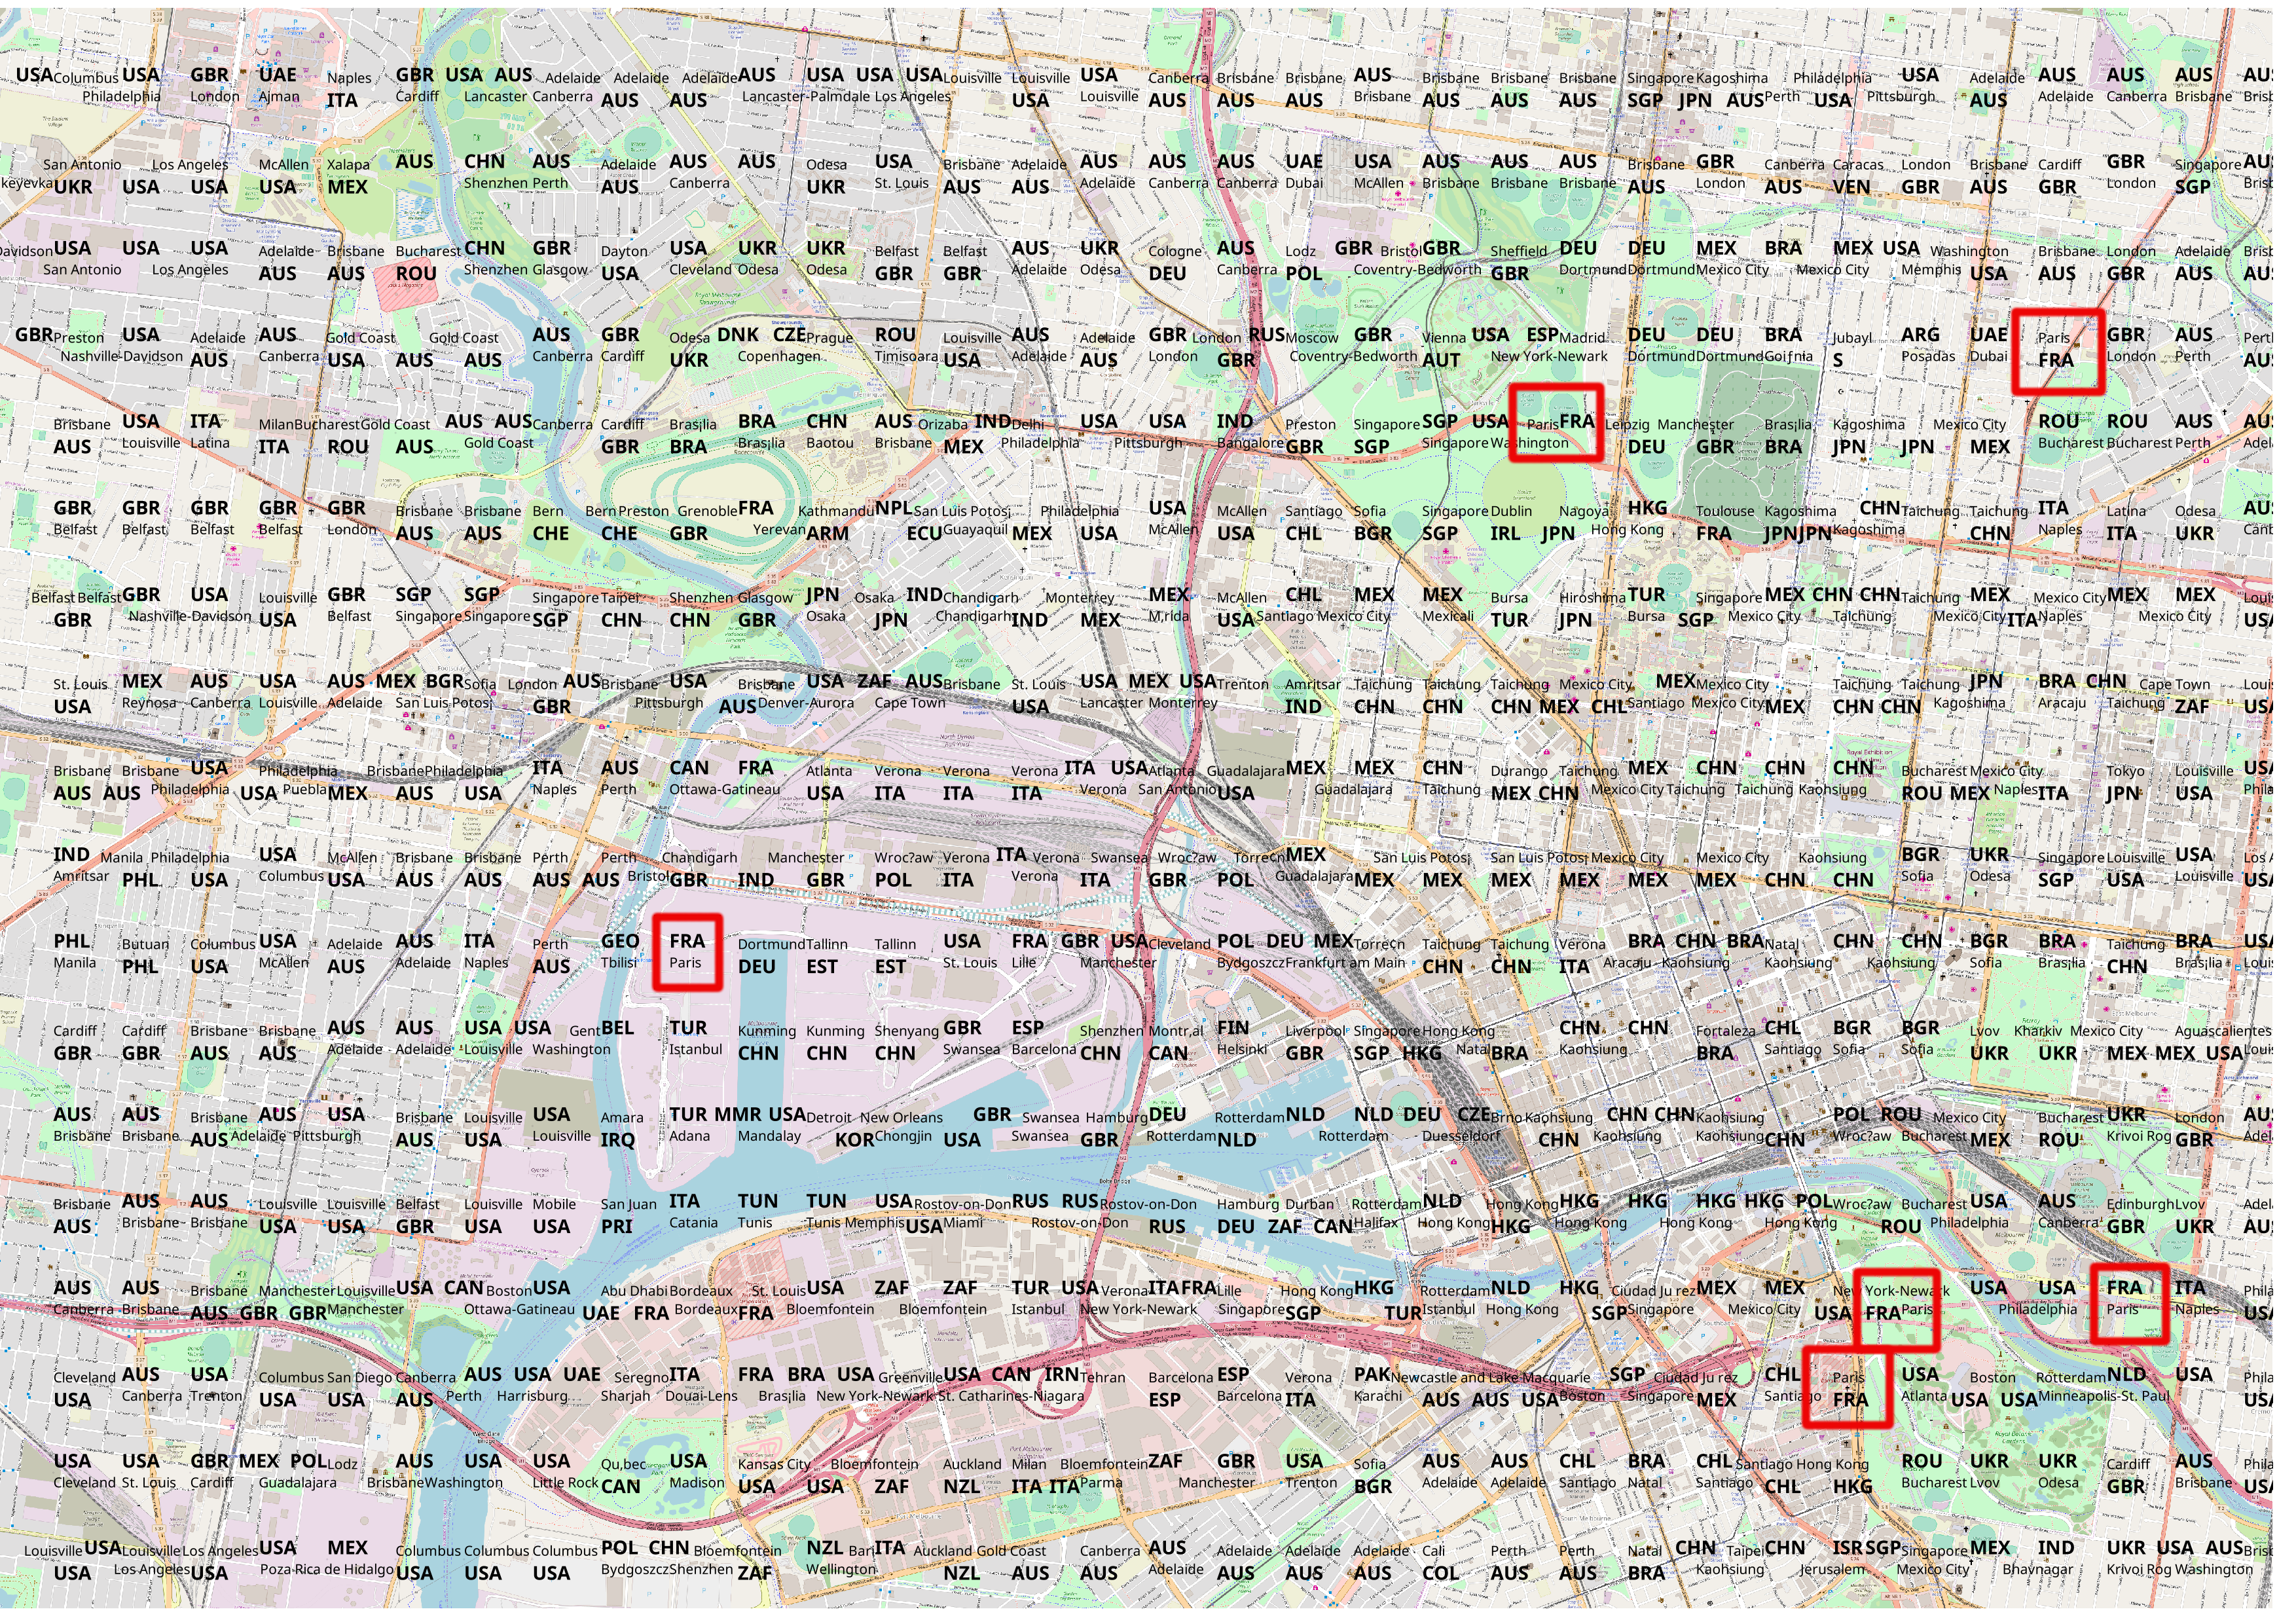
\includegraphics[scale=0.40]{Images/PlosOne/Fig7.png} 
\caption{\bf Predicted similar cities (showing three letter country code of city location) using the GM neural network for Melbourne evaluation locations. Detail of Melbourne CBD, with predictions of Paris highlighted in red squares. (TODO, is this figure readable enough?)}    
 \label{fig:melmapscbd}  
\end{figure} 

Fig \ref{fig:melsat} shows the top predicted cities (those predicted at a rate higher than 0.3\%) plotted against the Melbourne evaluation locations for the GS neural network. Paris-like locations are highlighted with a black star (1 location in total).  The other Australian cities show a strong grouping in the inner and outer suburbs while the CBD region shows no single strong grouping of regions or specific cities but with a range of predictions such as Miami, United States and Mendoza, Argentina. In Melbourne's far outer suburbs and rural areas, a wide mix is seen of North and South American (USA, Brazil, and Argentina), South African, European (Italy and Spain), and Mid-Eastern (Iran and Turkey) cities with small localized clusters of each. Only a single predictions of Paris, France has been made by the GS neural network for any evaluation location in Melbourne.

\begin{figure}[!htbp]
\centering    
\includegraphics[scale=0.16]{Images/PlosOne/Fig8.png} 
%\includegraphics[scale=0.20]{Images/MelbourneOverall_sat.png} 
%\includegraphics[scale=0.16]{Images/MelbourneOverallAbrev_sat.png} 
%\includegraphics[scale=0.16]{Images/SydneyOverallAbrev_sat.png}  
\caption{\bf Predicted similar cities using the GS neural network. Top predicted cities plotted using Fig \ref{fig:colorscheme} color scheme for Melbourne evaluation locations (top) and Sydney (bottom). Predicted Paris locations marked with black stars.} 
 \label{fig:melsat}  
\end{figure} 

Fig \ref{fig:melsat} shows the top predicted cities (those predicted at a rate higher than 0.3\%) plotted against the Sydney evaluation locations for the GS neural network. Paris-like locations are highlighted with a black star (although there are zero locations predicted). The overall predictions are dominated by cities in Brazil and other South American locations in the north and west and Ukraine in the south. Other Australian cities are only predicted in a few locations around the city. In the CBD, predictions continue to be dominated by Brazilian cities with some more scattered predictions of cities from Japan, Haiti, and Mexico. No predictions of Paris, France have been made by the GS neural network for any evaluation location in Sydney.

Fig \ref{fig:melstreet} shows the top predicted cities (those predicted at a rate higher than 0.3\%) plotted against the Melbourne evaluation locations for the GSV-BSV neural network. Paris-like locations are highlighted with a black star (13 locations in total). The overall predictions are dominated by other Australian cities scattered widely throughout the entire greater Melbourne area. The remaining evaluation locations show no strong groupings of any predicted countries or cities but some of the common predictions include cities from South Africa, New Zealand, the United States, and European countries. The CBD again shows a wide scattering of predictions with no single city or country dominating.

\begin{figure}[!htbp]
\centering    
\includegraphics[scale=0.16]{Images/PlosOne/Fig9.png} 
%\includegraphics[scale=0.16]{Images/MelbourneOverallAbrev_street.png} 
%\includegraphics[scale=0.16]{Images/SydneyOverallAbrev_street.png}  
\caption{\bf Predicted similar cities using the GSV-BSV neural network. Top predicted cities plotted using Fig \ref{fig:colorscheme} color scheme for Melbourne evaluation locations (top) and Sydney (bottom). Predicted Paris locations marked with black stars.}   
 \label{fig:melstreet}  
\end{figure} 

Fig \ref{fig:melstreet} shows the top predicted cities (those predicted at a rate higher than 0.3\%) plotted against the Sydney evaluation locations for the GSV-BSV neural network. Paris-like locations are highlighted with a black star (6 locations in total). The results are very similar to those in the Melbourne evaluation. Again, the overall predictions are dominated by other Australian cities scattered widely throughout the entire greater Sydney area. The remaining predicted results show no strong groupings of any predicted countries or cities but some of the common predictions include cities from the United States, New Zealand, South African, and a number of European countries. The CBD shows a similar scattering of predictions with no single city or country dominating (apart from other Australian cities). The total number of predicted `Paris-like` locations across all three neural networks for each city are presented in Table \ref{tab:melbournesydneyparis}.

\begin{table}[!htbp]
\caption{\bf How much are Melbourne and Sydney like Paris? \label{tab:melbournesydneyparis}}     
\begin{tabular}{ l  l l l  l}
 \hline    &  \multicolumn{2}{c}{\textbf{Melbourne}} & \multicolumn{2}{c}{\textbf{Sydney}}  \\  
\textbf{Neural network} & \textbf{Matches} & \textbf{\% matching}  & \textbf{Matches} & \textbf{\% matching}\\ \hline
GM & 70 & 0.3 & 99 & 0.4 \\ 
GS & 1 & 0.00004 & 0 & 0 \\ 
GSV-BSV & 13 & 0.06 & 6 & 0.04 \\ \hline
\end{tabular}
\end{table}


\section*{Discussion}\label{sec:discussion}
This study set out to answer the question is there a `Paris-end' of Melbourne or Sydney? As the results shows, we can conclusively state that neither Melbourne or Sydney have a strong case to claim that they are like Paris or have an extensive `Paris-end' of town. Using three different trained neural networks and three different sources of imagery, very few locations in Melbourne or Sydney are confused with Paris by the neural networks. 

However, in looking at the few locations that are deemed to be `Paris-like', there are a number of common characteristics that stand out. A gallery of all of the images for Melbourne and Sydney that the GM neural network found were similar to Paris are presented in Fig \ref{fig:gm_mel_gallery} and \ref{fig:gm_syd_gallery}. There are a number of common elements in these galleries. Many of these map images show large parklands (in green) embedded in the cities. Orange lines of public transport (rail and tram) are prominent in the majority of these images as well as large water bodies (in blue). Large arterial and trunk roads run nearby smaller (often curving) local roads, however these local roads tend to still be larger and do not reach the small intricate layouts of some Asian cities.





\begin{figure}[!htbp]
\centering   
\includegraphics[scale=0.14]{Images/PlosOne/Fig10.png}   
%\includegraphics[scale=0.12]{{Images/MelbourneLikeParis/maps/10229_7531_-37.903588,145.006012}.png}   
%\includegraphics[scale=0.12]{{Images/MelbourneLikeParis/maps/4266_2255_-37.755988,145.362412}.png}  
%\includegraphics[scale=0.12]{{Images/MelbourneLikeParis/maps/7498_4800_-37.824388,144.959212}.png}
%\includegraphics[scale=0.12]{{Images/MelbourneLikeParis/maps/10253_7555_-37.903588,145.092412}.png}   
%\includegraphics[scale=0.12]{{Images/MelbourneLikeParis/maps/4908_2610_-37.770388,145.063612}.png}  
%\includegraphics[scale=0.12]{{Images/MelbourneLikeParis/maps/7502_4804_-37.824388,144.973612}.png}
%\includegraphics[scale=0.12]{{Images/MelbourneLikeParis/maps/10484_7786_-37.914388,144.988012}.png}   
%\includegraphics[scale=0.12]{{Images/MelbourneLikeParis/maps/5222_5221_-37.777588,144.876412}.png}  
%\includegraphics[scale=0.12]{{Images/MelbourneLikeParis/maps/7563_4865_-37.824388,145.193212}.png}
%\includegraphics[scale=0.12]{{Images/MelbourneLikeParis/maps/11419_8721_-37.950388,145.290412}.png}   
%\includegraphics[scale=0.12]{{Images/MelbourneLikeParis/maps/5789_3091_-37.788388,144.941212}.png}  
%\includegraphics[scale=0.12]{{Images/MelbourneLikeParis/maps/7642_4944_-37.827988,144.955612}.png}
%\includegraphics[scale=0.12]{{Images/MelbourneLikeParis/maps/11727_9029_-37.964788,145.254412}.png}   
%\includegraphics[scale=0.12]{{Images/MelbourneLikeParis/maps/5790_3092_-37.788388,144.944812}.png}  
%\includegraphics[scale=0.12]{{Images/MelbourneLikeParis/maps/7659_4961_-37.827988,145.016812}.png}
%\includegraphics[scale=0.12]{{Images/MelbourneLikeParis/maps/12157_9459_-37.982788,145.132012}.png}   
%\includegraphics[scale=0.12]{{Images/MelbourneLikeParis/maps/5793_3095_-37.788388,144.955612}.png}  
%\includegraphics[scale=0.12]{{Images/MelbourneLikeParis/maps/7820_5122_-37.831588,145.067212}.png}
%\includegraphics[scale=0.12]{{Images/MelbourneLikeParis/maps/12332_9634_-37.989988,145.067212}.png}   
%\includegraphics[scale=0.12]{{Images/MelbourneLikeParis/maps/5794_3096_-37.788388,144.959212}.png}  
%\includegraphics[scale=0.12]{{Images/MelbourneLikeParis/maps/8090_5392_-37.838788,144.973612}.png}
%\includegraphics[scale=0.12]{{Images/MelbourneLikeParis/maps/12333_9635_-37.989988,145.070812}.png}   
%\includegraphics[scale=0.12]{{Images/MelbourneLikeParis/maps/5803_3105_-37.788388,144.991612}.png}  
%\includegraphics[scale=0.12]{{Images/MelbourneLikeParis/maps/8558_5860_-37.849588,145.135612}.png}
%\includegraphics[scale=0.12]{{Images/MelbourneLikeParis/maps/12425_9727_-37.993588,145.078012}.png}   
%\includegraphics[scale=0.12]{{Images/MelbourneLikeParis/maps/5976_3278_-37.791988,144.955612}.png}  
%\includegraphics[scale=0.12]{{Images/MelbourneLikeParis/maps/8580_5882_-37.849588,145.214812}.png}
%\includegraphics[scale=0.12]{{Images/MelbourneLikeParis/maps/14621_11923_-38.097988,145.139212}.png}  
%\includegraphics[scale=0.12]{{Images/MelbourneLikeParis/maps/5977_3279_-37.791988,144.959212}.png}  
%\includegraphics[scale=0.12]{{Images/MelbourneLikeParis/maps/8612_5914_-37.849588,145.330012}.png}
%\includegraphics[scale=0.12]{{Images/MelbourneLikeParis/maps/14622_11924_-38.097988,145.142812}.png}  
%\includegraphics[scale=0.12]{{Images/MelbourneLikeParis/maps/5995_3297_-37.791988,145.024012}.png}  
%\includegraphics[scale=0.12]{{Images/MelbourneLikeParis/maps/8648_5950_-37.853188,144.898012}.png}
%\includegraphics[scale=0.12]{{Images/MelbourneLikeParis/maps/15488_12790_-38.137588,145.261612}.png}  
%\includegraphics[scale=0.12]{{Images/MelbourneLikeParis/maps/6159_3461_-37.795588,144.955612}.png}  
%\includegraphics[scale=0.12]{{Images/MelbourneLikeParis/maps/8778_6080_-37.856788,144.854812}.png}
%\includegraphics[scale=0.12]{{Images/MelbourneLikeParis/maps/16106_13408_-38.166388,145.168012}.png}  
%\includegraphics[scale=0.12]{{Images/MelbourneLikeParis/maps/6478_3780_-37.802788,144.775612}.png}  
%\includegraphics[scale=0.12]{{Images/MelbourneLikeParis/maps/8791_6093_-37.856788,144.901612}.png}
%\includegraphics[scale=0.12]{{Images/MelbourneLikeParis/maps/1702_1701_-37.701988,144.887212}.png}    
%\includegraphics[scale=0.12]{{Images/MelbourneLikeParis/maps/6572_3874_-37.802788,145.114012}.png}  
%\includegraphics[scale=0.12]{{Images/MelbourneLikeParis/maps/9030_6332_-37.860388,145.322812}.png}
%\includegraphics[scale=0.12]{{Images/MelbourneLikeParis/maps/18281_15579_-38.256388,145.027612}.png}  
%\includegraphics[scale=0.12]{{Images/MelbourneLikeParis/maps/6783_4085_-37.806388,145.222012}.png}  
%\includegraphics[scale=0.12]{{Images/MelbourneLikeParis/maps/9071_6373_-37.863988,144.977212}.png}
%\includegraphics[scale=0.12]{{Images/MelbourneLikeParis/maps/1842_971_-37.705588,144.916012}.png}     
%\includegraphics[scale=0.12]{{Images/MelbourneLikeParis/maps/6884_4186_-37.809988,144.941212}.png}  
%\includegraphics[scale=0.12]{{Images/MelbourneLikeParis/maps/9073_6375_-37.863988,144.984412}.png}
%\includegraphics[scale=0.12]{{Images/MelbourneLikeParis/maps/1843_972_-37.705588,144.919612}.png}     
%\includegraphics[scale=0.12]{{Images/MelbourneLikeParis/maps/7202_4504_-37.817188,144.948412}.png}  
%\includegraphics[scale=0.12]{{Images/MelbourneLikeParis/maps/9192_6494_-37.867588,144.898012}.png}
%\includegraphics[scale=0.12]{{Images/MelbourneLikeParis/maps/18489_15785_-38.267188,145.096012}.png}  
%\includegraphics[scale=0.12]{{Images/MelbourneLikeParis/maps/7357_4659_-37.820788,144.970012}.png}  
%\includegraphics[scale=0.12]{{Images/MelbourneLikeParis/maps/9196_6498_-37.867588,144.912412}.png}
%\includegraphics[scale=0.12]{{Images/MelbourneLikeParis/maps/19102_16395_-38.303188,144.995212}.png}  
%\includegraphics[scale=0.12]{{Images/MelbourneLikeParis/maps/7358_4660_-37.820788,144.973612}.png}  
%\includegraphics[scale=0.12]{{Images/MelbourneLikeParis/maps/9428_6730_-37.874788,144.991612}.png}
%\includegraphics[scale=0.12]{{Images/MelbourneLikeParis/maps/2729_2728_-37.727188,144.858412}.png}    
%\includegraphics[scale=0.12]{{Images/MelbourneLikeParis/maps/7359_4661_-37.820788,144.977212}.png}  
%\includegraphics[scale=0.12]{{Images/MelbourneLikeParis/maps/9465_6767_-37.874788,145.124812}.png}
%\includegraphics[scale=0.12]{{Images/MelbourneLikeParis/maps/2741_2740_-37.727188,144.901612}.png}    
%\includegraphics[scale=0.12]{{Images/MelbourneLikeParis/maps/7416_4718_-37.820788,145.182412}.png}  
%\includegraphics[scale=0.12]{{Images/MelbourneLikeParis/maps/9537_6839_-37.878388,144.995212}.png}
%\includegraphics[scale=0.12]{{Images/MelbourneLikeParis/maps/2879_1521_-37.730788,144.818812}.png}    
%\includegraphics[scale=0.12]{{Images/MelbourneLikeParis/maps/7417_4719_-37.820788,145.186012}.png}  
%\includegraphics[scale=0.12]{{Images/MelbourneLikeParis/maps/9837_7139_-37.889188,144.793612}.png}
%\includegraphics[scale=0.12]{{Images/MelbourneLikeParis/maps/3063_1622_-37.734388,144.890812}.png}    
%\includegraphics[scale=0.12]{{Images/MelbourneLikeParis/maps/7418_4720_-37.820788,145.189612}.png}
%\includegraphics[scale=0.12]{{Images/MelbourneLikeParis/maps/3382_3381_-37.741588,144.797212}.png}    
%\includegraphics[scale=0.12]{{Images/MelbourneLikeParis/maps/7419_4721_-37.820788,145.193212}.png}
\caption{\bf Gallery of `Paris-like` locations in Melbourne using the GM neural network.}    
 \label{fig:gm_mel_gallery} 
\end{figure} 





% \begin{figure}[!htbp]
% \centering    
% \includegraphics[scale=0.50]{Images/MelbourneLikeParis/Melbourne_maps_gallery.png} 
% \caption{Gallery of `Paris-like` locations in Melbourne using the GM neural network.}    
%  \label{fig:gm_mel_gallery}  
% \end{figure} 

\begin{figure}[!htbp]
\centering   
\includegraphics[scale=0.12]{Images/PlosOne/Fig11.png}   
% %\includegraphics[scale=0.50]{Images/SydneyLikeParis/Sydney_maps_gallery.png} 
%\includegraphics[scale=0.12]{{Images/SydneyLikeParis/maps/10210_10209_-33.809806,151.090242}.png}
%\includegraphics[scale=0.12]{{Images/SydneyLikeParis/maps/14890_14889_-33.907006,151.104642}.png}
%\includegraphics[scale=0.12]{{Images/SydneyLikeParis/maps/21903_21902_-34.076206,150.820242}.png}
%\includegraphics[scale=0.12]{{Images/SydneyLikeParis/maps/10212_10211_-33.809806,151.097442}.png}
%\includegraphics[scale=0.12]{{Images/SydneyLikeParis/maps/15067_15066_-33.910606,151.119042}.png}
%\includegraphics[scale=0.12]{{Images/SydneyLikeParis/maps/22834_22833_-34.101406,151.093842}.png}
%\includegraphics[scale=0.12]{{Images/SydneyLikeParis/maps/10234_10233_-33.809806,151.180242}.png}
%\includegraphics[scale=0.12]{{Images/SydneyLikeParis/maps/15068_15067_-33.910606,151.122642}.png}
%\includegraphics[scale=0.12]{{Images/SydneyLikeParis/maps/23380_23379_-34.119406,150.993042}.png}
%\includegraphics[scale=0.12]{{Images/SydneyLikeParis/maps/10418_10417_-33.813406,151.180242}.png}
%\includegraphics[scale=0.12]{{Images/SydneyLikeParis/maps/15072_15071_-33.910606,151.137042}.png}
%\includegraphics[scale=0.12]{{Images/SydneyLikeParis/maps/3843_3842_-33.676606,151.306242}.png}
%\includegraphics[scale=0.12]{{Images/SydneyLikeParis/maps/10419_10418_-33.813406,151.183842}.png}
%\includegraphics[scale=0.12]{{Images/SydneyLikeParis/maps/15233_15232_-33.914206,151.093842}.png}
%\includegraphics[scale=0.12]{{Images/SydneyLikeParis/maps/4136_4135_-33.683806,151.259442}.png}
%\includegraphics[scale=0.12]{{Images/SydneyLikeParis/maps/10506_10505_-33.817006,150.849042}.png}
%\includegraphics[scale=0.12]{{Images/SydneyLikeParis/maps/15234_15233_-33.914206,151.097442}.png}
%\includegraphics[scale=0.12]{{Images/SydneyLikeParis/maps/4962_4961_-33.701806,151.306242}.png}
%\includegraphics[scale=0.12]{{Images/SydneyLikeParis/maps/10598_10597_-33.817006,151.183842}.png}
%\includegraphics[scale=0.12]{{Images/SydneyLikeParis/maps/15388_15387_-33.917806,151.029042}.png}
%\includegraphics[scale=0.12]{{Images/SydneyLikeParis/maps/5531_5530_-33.716206,150.960642}.png}
%\includegraphics[scale=0.12]{{Images/SydneyLikeParis/maps/10600_10599_-33.817006,151.191042}.png}
%\includegraphics[scale=0.12]{{Images/SydneyLikeParis/maps/15588_15587_-33.921406,151.133442}.png}
%\includegraphics[scale=0.12]{{Images/SydneyLikeParis/maps/5726_5725_-33.719806,151.111842}.png}
%\includegraphics[scale=0.12]{{Images/SydneyLikeParis/maps/10754_10753_-33.820606,151.115442}.png}
%\includegraphics[scale=0.12]{{Images/SydneyLikeParis/maps/15944_15943_-33.928606,151.169442}.png}
%\includegraphics[scale=0.12]{{Images/SydneyLikeParis/maps/5893_5892_-33.723406,151.097442}.png}
%\includegraphics[scale=0.12]{{Images/SydneyLikeParis/maps/10774_10773_-33.820606,151.191042}.png}
%\includegraphics[scale=0.12]{{Images/SydneyLikeParis/maps/16291_16290_-33.935806,151.147842}.png}
%\includegraphics[scale=0.12]{{Images/SydneyLikeParis/maps/5894_5893_-33.723406,151.101042}.png}
%\includegraphics[scale=0.12]{{Images/SydneyLikeParis/maps/10906_10905_-33.824206,151.007442}.png}
%\includegraphics[scale=0.12]{{Images/SydneyLikeParis/maps/16448_16447_-33.939406,151.075842}.png}
%\includegraphics[scale=0.12]{{Images/SydneyLikeParis/maps/5899_5898_-33.723406,151.119042}.png}
%\includegraphics[scale=0.12]{{Images/SydneyLikeParis/maps/11284_11283_-33.831406,151.126242}.png}
%\includegraphics[scale=0.12]{{Images/SydneyLikeParis/maps/16465_16464_-33.939406,151.137042}.png}
%\includegraphics[scale=0.12]{{Images/SydneyLikeParis/maps/6601_6600_-33.737806,151.137042}.png}
%\includegraphics[scale=0.12]{{Images/SydneyLikeParis/maps/11398_11397_-33.835006,150.885042}.png}
%\includegraphics[scale=0.12]{{Images/SydneyLikeParis/maps/16481_16480_-33.939406,151.194642}.png}
%\includegraphics[scale=0.12]{{Images/SydneyLikeParis/maps/6844_6843_-33.745006,150.672642}.png}
%\includegraphics[scale=0.12]{{Images/SydneyLikeParis/maps/11475_11474_-33.835006,151.209042}.png}
%\includegraphics[scale=0.12]{{Images/SydneyLikeParis/maps/16657_16656_-33.943006,151.191042}.png}
%\includegraphics[scale=0.12]{{Images/SydneyLikeParis/maps/7405_7404_-33.755806,150.719442}.png}
%\includegraphics[scale=0.12]{{Images/SydneyLikeParis/maps/11476_11475_-33.835006,151.212642}.png}
%\includegraphics[scale=0.12]{{Images/SydneyLikeParis/maps/17176_17175_-33.953806,151.137042}.png}
%\includegraphics[scale=0.12]{{Images/SydneyLikeParis/maps/7588_7587_-33.759406,150.719442}.png}
%\includegraphics[scale=0.12]{{Images/SydneyLikeParis/maps/11652_11651_-33.838606,151.212642}.png}
%\includegraphics[scale=0.12]{{Images/SydneyLikeParis/maps/17305_17304_-33.957406,150.985842}.png}
%\includegraphics[scale=0.12]{{Images/SydneyLikeParis/maps/7640_7639_-33.759406,150.906642}.png}
%\includegraphics[scale=0.12]{{Images/SydneyLikeParis/maps/11785_11784_-33.842206,151.021842}.png}
%\includegraphics[scale=0.12]{{Images/SydneyLikeParis/maps/17346_17345_-33.957406,151.133442}.png}
%\includegraphics[scale=0.12]{{Images/SydneyLikeParis/maps/8005_8004_-33.766606,150.903042}.png}
%\includegraphics[scale=0.12]{{Images/SydneyLikeParis/maps/11789_11788_-33.842206,151.036242}.png}
%\includegraphics[scale=0.12]{{Images/SydneyLikeParis/maps/17514_17513_-33.961006,151.133442}.png}
%\includegraphics[scale=0.12]{{Images/SydneyLikeParis/maps/8168_8167_-33.770206,150.831042}.png}
%\includegraphics[scale=0.12]{{Images/SydneyLikeParis/maps/12115_12114_-33.849406,151.032642}.png}
%\includegraphics[scale=0.12]{{Images/SydneyLikeParis/maps/17664_17663_-33.964606,151.086642}.png}
%\includegraphics[scale=0.12]{{Images/SydneyLikeParis/maps/8169_8168_-33.770206,150.834642}.png}
%\includegraphics[scale=0.12]{{Images/SydneyLikeParis/maps/12454_12453_-33.856606,151.065042}.png}
%\includegraphics[scale=0.12]{{Images/SydneyLikeParis/maps/17665_17664_-33.964606,151.090242}.png}
%\includegraphics[scale=0.12]{{Images/SydneyLikeParis/maps/8188_8187_-33.770206,150.903042}.png}
%\includegraphics[scale=0.12]{{Images/SydneyLikeParis/maps/12622_12621_-33.860206,151.079442}.png}
%\includegraphics[scale=0.12]{{Images/SydneyLikeParis/maps/17666_17665_-33.964606,151.093842}.png}
%\includegraphics[scale=0.12]{{Images/SydneyLikeParis/maps/8260_8259_-33.770206,151.162242}.png}
%\includegraphics[scale=0.12]{{Images/SydneyLikeParis/maps/12941_12940_-33.867406,151.079442}.png}
%\includegraphics[scale=0.12]{{Images/SydneyLikeParis/maps/17831_17830_-33.968206,151.097442}.png}
%\includegraphics[scale=0.12]{{Images/SydneyLikeParis/maps/8261_8260_-33.770206,151.165842}.png}
%\includegraphics[scale=0.12]{{Images/SydneyLikeParis/maps/12945_12944_-33.867406,151.093842}.png}
%\includegraphics[scale=0.12]{{Images/SydneyLikeParis/maps/17971_17970_-33.971806,151.029042}.png}
%\includegraphics[scale=0.12]{{Images/SydneyLikeParis/maps/8352_8351_-33.773806,150.838242}.png}
%\includegraphics[scale=0.12]{{Images/SydneyLikeParis/maps/13085_13084_-33.871006,151.000242}.png}
%\includegraphics[scale=0.12]{{Images/SydneyLikeParis/maps/18015_18014_-33.971806,151.245042}.png}
%\includegraphics[scale=0.12]{{Images/SydneyLikeParis/maps/8442_8441_-33.773806,151.162242}.png}
%\includegraphics[scale=0.12]{{Images/SydneyLikeParis/maps/13109_13108_-33.871006,151.086642}.png}
%\includegraphics[scale=0.12]{{Images/SydneyLikeParis/maps/18016_18015_-33.971806,151.248642}.png}
%\includegraphics[scale=0.12]{{Images/SydneyLikeParis/maps/8804_8803_-33.781006,151.173042}.png}
%\includegraphics[scale=0.12]{{Images/SydneyLikeParis/maps/13133_13132_-33.871006,151.191042}.png}
%\includegraphics[scale=0.12]{{Images/SydneyLikeParis/maps/18246_18245_-33.979006,150.921042}.png}
%\includegraphics[scale=0.12]{{Images/SydneyLikeParis/maps/8832_8831_-33.781006,151.281042}.png}
%\includegraphics[scale=0.12]{{Images/SydneyLikeParis/maps/13240_13239_-33.874606,150.957042}.png}
%\includegraphics[scale=0.12]{{Images/SydneyLikeParis/maps/18413_18412_-33.982606,150.996642}.png}
%\includegraphics[scale=0.12]{{Images/SydneyLikeParis/maps/8893_8892_-33.784606,150.845442}.png}
%\includegraphics[scale=0.12]{{Images/SydneyLikeParis/maps/13248_13247_-33.874606,150.985842}.png}
%\includegraphics[scale=0.12]{{Images/SydneyLikeParis/maps/19690_19689_-34.018606,150.831042}.png}
%\includegraphics[scale=0.12]{{Images/SydneyLikeParis/maps/8993_8992_-33.784606,151.205442}.png}
%\includegraphics[scale=0.12]{{Images/SydneyLikeParis/maps/13603_13602_-33.881806,150.975042}.png}
%\includegraphics[scale=0.12]{{Images/SydneyLikeParis/maps/20215_20214_-34.029406,151.183842}.png}
%\includegraphics[scale=0.12]{{Images/SydneyLikeParis/maps/9292_9291_-33.791806,150.993042}.png}
%\includegraphics[scale=0.12]{{Images/SydneyLikeParis/maps/1377_1376_-33.579406,151.295442}.png}
%\includegraphics[scale=0.12]{{Images/SydneyLikeParis/maps/20496_20495_-34.036606,151.104642}.png}
%\includegraphics[scale=0.12]{{Images/SydneyLikeParis/maps/9856_9855_-33.802606,151.090242}.png}
%\includegraphics[scale=0.12]{{Images/SydneyLikeParis/maps/14046_14045_-33.889006,151.270242}.png}
%\includegraphics[scale=0.12]{{Images/SydneyLikeParis/maps/21118_21117_-34.054606,150.820242}.png}
%\includegraphics[scale=0.12]{{Images/SydneyLikeParis/maps/9974_9973_-33.806206,150.881442}.png}
%\includegraphics[scale=0.12]{{Images/SydneyLikeParis/maps/14136_14135_-33.892606,150.942642}.png}
%\includegraphics[scale=0.12]{{Images/SydneyLikeParis/maps/21514_21513_-34.065406,150.816642}.png}
%\includegraphics[scale=0.12]{{Images/SydneyLikeParis/maps/9975_9974_-33.806206,150.885042}.png}
%\includegraphics[scale=0.12]{{Images/SydneyLikeParis/maps/14561_14560_-33.899806,151.187442}.png}
%\includegraphics[scale=0.12]{{Images/SydneyLikeParis/maps/2164_2163_-33.629806,151.176642}.png}
%\includegraphics[scale=0.12]{{Images/SydneyLikeParis/maps/9976_9975_-33.806206,150.888642}.png}
\caption{\bf Gallery of `Paris-like` locations in Sydney using the GM neural network.}    
 \label{fig:gm_syd_gallery}  
\end{figure} 

As the GSV-BSV neural network only picked Paris for 0.062\% of the evaluated locations for Melbourne and 0.040\% for Sydney, it can be stated that from a visual street-level view, there is almost nothing about either Melbourne or Sydney that is visually similar to Paris using this type of imagery. In the galleries of `Paris-like' images for Melbourne and Sydney (Fig \ref{fig:gsv_mel_gallery} and  \ref{fig:gsv_syd_gallery}), it can only be inferred that perhaps street trees (of a certain type) are an important part of what makes Paris look like Paris.

\begin{figure}[!htbp]
\centering    
\includegraphics[scale=0.35]{Images/PlosOne/Fig12.png}  
% %\includegraphics[scale=0.50]{Images/MelbourneLikeParis/Melbourne_streetview_gallery.png} 
%\includegraphics[scale=0.35]{{Images/MelbourneLikeParis/street/13476_-38.040388019999796_145.135611799999990}.jpg}  
%\includegraphics[scale=0.35]{{Images/MelbourneLikeParis/street/6376_-37.799188019999747_145.074411800000010}.jpg}
%\includegraphics[scale=0.35]{{Images/MelbourneLikeParis/street/14548_-38.094388019999712_145.142811800000000}.jpg}  
%\includegraphics[scale=0.35]{{Images/MelbourneLikeParis/street/6929_-37.809988019999821_145.103211800000170}.jpg}
%\includegraphics[scale=0.35]{{Images/MelbourneLikeParis/street/2918_-37.730788019999693_144.959211800000050}.jpg}   
%\includegraphics[scale=0.35]{{Images/MelbourneLikeParis/street/7346_-37.820788019999725_144.930411800000000}.jpg}
%\includegraphics[scale=0.35]{{Images/MelbourneLikeParis/street/4706_-37.766788019999751_144.988011799999980}.jpg}   
%\includegraphics[scale=0.35]{{Images/MelbourneLikeParis/street/8234_-37.842388019999817_144.984411800000090}.jpg}
%\includegraphics[scale=0.35]{{Images/MelbourneLikeParis/street/5796_-37.788388019999729_144.966411800000060}.jpg}   
%\includegraphics[scale=0.35]{{Images/MelbourneLikeParis/street/8345_-37.845988019999822_144.836811800000190}.jpg}
%\includegraphics[scale=0.35]{{Images/MelbourneLikeParis/street/5818_-37.788388019999729_145.045611800000070}.jpg}   
%\includegraphics[scale=0.35]{{Images/MelbourneLikeParis/street/9751_-37.885588019999659_145.009611800000020}.jpg}
%\includegraphics[scale=0.35]{{Images/MelbourneLikeParis/street/5975_-37.791988019999792_144.952011800000150}.jpg}
\caption{\bf Gallery of `Paris-like` locations in Melbourne using the GSV-BSV neural network.}    
 \label{fig:gsv_mel_gallery}  
\end{figure} 

\begin{figure}[!htbp]
\centering    
\includegraphics[scale=0.35]{Images/PlosOne/Fig13.png}  
% %\includegraphics[scale=0.50]{Images/SydneyLikeParis/Sydney_streetview_gallery.png} 
%\includegraphics[scale=0.35]{{Images/SydneyLikeParis/street/10368_-33.813405549999914_151.000242100000040}.jpg}  
%\includegraphics[scale=0.35]{{Images/SydneyLikeParis/street/13489_-33.878205549999905_151.209042099999920}.jpg}
%\includegraphics[scale=0.35]{{Images/SydneyLikeParis/street/11740_-33.842205549999903_150.859842099999920}.jpg}  
%\includegraphics[scale=0.35]{{Images/SydneyLikeParis/street/14039_-33.889005549999865_151.245042099999980}.jpg}
%\includegraphics[scale=0.35]{{Images/SydneyLikeParis/street/13311_-33.874605549999899_151.212642100000040}.jpg}  
%\includegraphics[scale=0.35]{{Images/SydneyLikeParis/street/15275_-33.914205549999849_151.245042099999980}.jpg}
\caption{\bf Gallery of `Paris-like` locations in Sydney using the GSV-BSV neural network.}    
 \label{fig:gsv_syd_gallery}  
\end{figure} 



Finally, using the GS neural network, none of the evaluated locations for Sydney and only one location for Melbourne were predicted to be `Paris-like'. This means from an overhead remote sensing point of view, there is nothing about either Melbourne or Sydney that shares any similar visual characteristics with Paris.

Despite these disappointing results (at least from the standpoint of some Australian cities aspiring to be mistaken for the `City of Light'), this analysis reveals a number of exciting possibilities for using neural networks to analyse urban areas. This fundamental methodology can be used to look at many different aspects of cities and understand what elements of their urban design leads them to work in different ways, using easily obtained and globally consistent imagery. 

The GM neural network used in this study has also been used to cluster world cities and examine how the make up of cities in each cluster (based on urban green space, amounts and types of public transport, and road networks) impact health outcomes in those types of cities (CITE TO LANCET). 

As seen in the unsuccessful attempt to find significant areas of `Paris-like' locations in Melbourne or Sydney, certain characteristics stand out as strongly influencing how each city fits into a specific typology and of other similar cities in those same typologies. Using the GM neural network approach, urban form can be evaluated. Characteristics that will be influential in grouping cities with a particular typology will include extents and types of public transportation, urban green space size and embeddedness, road network structure, water body inclusion and integration, amounts of informal unplanned open space, and density and topology influences on city structure. Some of the features included in the GM imagery that made cities `Paris-like' were a higher density of trains and trams, large broad sections of urban green space, and an integration of urban green space and waterways.


Using remote sensing (satellite imagery) of urban areas, natural characteristics will feature more predominantly in classifying locations within a particular typology. In Fig \ref{fig:satimages}a, satellite imagery of Melbourne shows a number of colour and terrain similarities with its top 6, namely Adelaide, Australia; Campinas, Brazil; Jundia\'{i}, Brazil; Miami, USA; Provo, USA; and Wellington, NZ (all shown in Fig \ref{fig:satimages}). Perhaps showing that natural characteristics are more influential to what the GS neural networks think make cities similar than the characteristics of built urban form highlighted by the GM neural network.


\begin{figure}[!htbp]
\centering    
\includegraphics[scale=0.35]{Images/PlosOne/Fig14.png} 
%a) \includegraphics[trim = 50mm 50mm 50mm 50mm, clip, scale=0.18]{Images/GoogleSatelliteCities/Melbourne2.png} 
%\\ b) \includegraphics[trim = 50mm 50mm 50mm 50mm, clip, scale=0.18]{Images/GoogleSatelliteCities/Adelaide2.png} 
%c) \includegraphics[trim = 50mm 50mm 50mm 50mm, clip, scale=0.18]{Images/GoogleSatelliteCities/Campinas2.png} 
%\\ d) \includegraphics[trim = 50mm 50mm 50mm 50mm, clip, scale=0.18]{Images/GoogleSatelliteCities/Jundai2.png} 
%e) \includegraphics[trim = 50mm 50mm 50mm 50mm, clip, scale=0.18]{Images/GoogleSatelliteCities/Maimi2.png} 
%\\ f) \includegraphics[trim = 50mm 50mm 50mm 50mm, clip, scale=0.18]{Images/GoogleSatelliteCities/Provo2.png} 
%g) \includegraphics[trim = 50mm 50mm 50mm 50mm, clip, scale=0.18]{Images/GoogleSatelliteCities/Wellington2.png} 
 \caption{\bf Satellite imagery of (a) Melbourne, Australia, (b) Adelaide, Australia, (c) Campinas, Brazil, (d) Jundia\'{i}, Brazil, (e) Miami, USA, (f) Provo, USA, and (g) Wellington, NZ \cite{GoogleStatic2017}.}    
 \label{fig:satimages}  
\end{figure} 
%CITE DOER%
Finally, in examining the results from the GSV-BSV neural network evaluation, this micro-scaled level of imagery would arguably capture the visual geography that most people would say `this is what makes Paris look like Paris'. Or in the case of this study, these visual elements are what makes Melbourne or Sydney look like Paris. But as \cite{Doersch2012} found in trying to answer the question of `What makes Paris look like Paris?', overall this answer is not based on a small number of famous iconic landmarks (i.e. the Eiffel Tower, the Louvre, etc.) but on a vast array of widespread smaller features. These features include elements such as cast-iron railings on balconies, grid-like balcony arrangements, distinctive street signs, streetlamps on pedestals, window balustrades, and Parisian doorways. Other factors that make the two Australian cities less Paris-like are the types of urban vegetation as well as amounts. For example, Paris has a much lower Green View Index (the amount of vegetation visible at a street level), 8.8\% compared to Sydney's 25.9\% \cite{Li2015}. The colour and quantity of street level vegetation will be highly influential in the neural network's predictions. Of all these micro-scaled visual elements, neither Melbourne or Sydney contain enough of these elements to truly have a `Paris-end' of town.



\section*{Conclusion}\label{sec:conclusion}

In this study, we have conclusively answered the question, does Melbourne or Sydney have a `Paris-end' of town with a definitive `no'. Using millions of images of thousands of cities, our three trained neural networks concluded that at best, Sydney could be considered only 0.4\% `Paris-like` while Melbourne can only boast 0.3\%. In addition, our tools now let any city in the world answer the age-old question for themselves, do we have a `Paris-end' of town?

But in answering this question, we have also demonstrated some new techniques for assessing urban typologies based on a number of different urban characteristics. Using three different sources of imagery (street maps, satellite imagery, and street view level imagery), our trained neural networks are able to identify commonalities between a wide number of cities and allow us to see these cities in entirely new ways. Importantly, we have demonstrated that results are sensitive to differences in imagery input information, which must be considered in future applications. 



%Using the GM neural network, urban features such as wide broad green spaces, a high level of public transport, the form and scale of the road networks, and topography and natural features become influential in grouping cities into clusters. Using the GS neural network, natural characteristics become to dominate the grouping of these city clusters. Finally, with the GSV-BSV neural network, micro-scaled visual geographical features (road widths, urban vegetation, building styles, etc.) become the dominant influence on how different world cities are clustered together. This clustering based on various elements of urban form can then allow further analysis in how the urban form influences outcomes with in these areas. Such areas of study can include health outcomes, transportation options, and many other topics. 



\nolinenumbers

% Either type in your references using
% \begin{thebibliography}{}
% \bibitem{}
% Text
% \end{thebibliography}
%
% or
%
% Compile your BiBTeX database using our plos2015.bst
% style file and paste the contents of your .bbl file
% here. See http://journals.plos.org/plosone/s/latex for 
% step-by-step instructions.
% 
\begin{thebibliography}{}

 %\bibliographystyle{plos2015}
 %\bibliography{library}


\bibitem{UNDESA2015}
UNDESA. {World Urbanization Prospects: The 2014 Revision}; 2015.
\newblock https://esa.un.org/unpd/wup/.

\bibitem{WHO2016}
WHO. {World Health Organization | Urban Population Growth}; 2016.
\newblock
  http://www.who.int/gho/urban{\_}health/situation{\_}trends/urban{\_}population{\_}growth{\_}text/en/.

\bibitem{UN2014}
{United Nations}. {Department of Economic and Social Affairs, Population
  Division, World Urbanization Prospects: The 2014 Revision, CD-ROM Edition};
  2014.

\bibitem{ABS2008}
ABS. {3222.0 - Population Projections, Australia, 2012 (base) to 2101.
  Australian Bureau of Statistics.}; 2013.
\newblock http://www.abs.gov.au/Ausstats/abs@.nsf/mf/3222.0.

\bibitem{CommonwealthofAustralia2010}
{Commonwealth of Australia}. {Australia to 2050: future challenges}; 2010.
\newblock http://www.treasury.gov.au/igr/igr2010.
\newblock Available from: \url{http://www.treasury.gov.au/igr/igr2010}.

\bibitem{ATAP2016}
{Commonwealth of Australia}. {Australian Transport Assessment and Planning
  Guidelines: F0.2 Integrated Transport and Land Use Planning. Australian
  Transport Assessment and Planning (ATAP) Steering Committee.}; 2016.

\bibitem{SAustralia2015}
{Government of South Australia}. {Building a Stronger South Australia: The
  Integrated Transport and Land Use Plan, July 2015}; 2015.

\bibitem{Currie2007}
Currie G, Senbergs Z.
\newblock {Exploring forced car ownership in metropolitan Melbourne}.
\newblock 30th Australasian Transport Research Forum. 2007;.

\bibitem{Dodson2008}
Dodson J, Sipe N.
\newblock {Shocking the suburbs: Urban location, homeownership and oil
  vulnerability in the Australian City}.
\newblock Housing Studies. 2008;23(3):377--401.
\newblock doi:{10.1080/02673030802015619}.

\bibitem{Heesch2014}
Heesch KC, Giles-Corti B, Turrell G.
\newblock {Cycling for transport and recreation: Associations with
  socio-economic position, environmental perceptions, and psychological
  disposition}.
\newblock Preventive Medicine. 2014;63:29--35.

\bibitem{Daley2011}
Daley M, Rissel C.
\newblock {Perspectives and images of cycling as a barrier or facilitator of
  cycling}.
\newblock Transport Policy. 2011;18(1):211--216.
\newblock doi:{10.1016/j.tranpol.2010.08.004}.

\bibitem{Cepeda2016}
Cepeda M, Schoufour J, Freak-poli R, Koolhaas CM, Dhana K, Bramer WM, et~al.
\newblock {Levels of ambient air pollution according to mode of transport: a
  systematic review}.
\newblock Lancet Public Health. 2016;2(1):e23--e34.
\newblock doi:{10.1016/S2468-2667(16)30021-4}.

\bibitem{MingWen2008}
{Ming Wen} L, Rissel C.
\newblock {Inverse associations between cycling to work, public transport, and
  overweight and obesity: Findings from a population based study in Australia}.
\newblock Preventive Medicine. 2008;46(1):29--32.
\newblock doi:{10.1016/j.ypmed.2007.08.009}.

\bibitem{Norman2006}
Norman J, MacLean HL, Kennedy CA.
\newblock {Comparing High and Low Residential Density : Life-Cycle Analysis of
  Energy Use and Greenhouse Gas Emissions}.
\newblock Journal of Urban Planning and Development. 2006;(March):10--21.

\bibitem{Copenhagen2017b}
{City of Copenhagen}. {Copenhagen City of Cyclists: The Bicycle Account 2016};
  2017.

\bibitem{Kaplan2014}
Kaplan S, Vavatsoulas K, Prato CG.
\newblock {Aggravating and mitigating factors associated with cyclist injury
  severity in Denmark}.
\newblock Journal of Safety Research. 2014;50:75--82.
\newblock doi:{10.1016/j.jsr.2014.03.012}.

\bibitem{Andersen2000}
Andersen LB, Schnohr P, Schroll M, Hein HO.
\newblock {All-cause mortality associated with physical activity during leisure
  time, work, sports, and cycling to work}.
\newblock Arch Intern Med. 2000;160(11):1621--1628.
\newblock doi:{10.1001/archinte.160.11.1621}.

\bibitem{Giles-corti2016}
Giles-corti B, Vernez-Moudon A, Reis R, Turrell G, Dannenberg AL, Badland H,
  et~al.
\newblock {Urban design, transport, and health 1 City planning and population
  health: a global challenge}.
\newblock The Lancet. 2016;6736(16):1--13.
\newblock doi:{10.1016/S0140-6736(16)30066-6}.

\bibitem{Kleinert2016}
Kleinert S, Horton R.
\newblock {Urban design: an important future force for health and wellbeing}.
\newblock The Lancet. 2016;6736(16):1--11.

\bibitem{Goenka2016}
Goenka S, Andersen LB.
\newblock {Urban design and transport to promote healthy lives}.
\newblock The Lancet. 2016;6736(16):8--10.
\newblock doi:{10.1016/S0140-6736(16)31580-X}.

\bibitem{Zapata-Diomedi2017}
Zapata-Diomedi B, Knibbs LD, Ware RS, Heesch KC, Tainio M, Woodcock J, et~al.
\newblock {A shift from motorised travel to active transport: What are the
  potential health gains for an Australian city?}
\newblock PLoS ONE. 2017;12(10):1--21.
\newblock doi:{10.1371/journal.pone.0184799}.

\bibitem{Anholt2006}
Anholt S.
\newblock {The Anholt-GMI City Brands Index: How the world sees the world's
  cities}.
\newblock Place Branding. 2006;2(1):18--31.

\bibitem{Williams2010}
Williams R.
\newblock {'Tower plans cast shadow over Collins Street's 'Paris end''}.
\newblock The Age. 2010;May 10:Online.

\bibitem{Wilden2013}
Wilden N.
\newblock {'France-Soir: A bite of Paris on the Yarra'}.
\newblock The Australian. 2013;December 2:Online.

\bibitem{Doersch2012}
Doersch C, Singh S, Gupta A, Sivic J, Efros A.
\newblock {What Makes Paris Look like Paris?}
\newblock ACM Transactions on Graphics, Association for Computing Machinery.
  2012;31(4).

\bibitem{Bishop1995}
Bishop CM.
\newblock {Neural Networks for Pattern Recognition}.
\newblock Oxford: Clarendon Press; 1995.

\bibitem{Samarasinghe2016}
Samarasinghe S.
\newblock {Neural Networks for Applied Sciences and Engineering: From
  Fundamentals to Complex Pattern Recognition}.
\newblock CRC Press; 2016.

\bibitem{Graupe2013}
Graupe D.
\newblock {Advanced Series in Circuits and Systems: Volume 7 Principles of
  Artificial Neural Networks}.
\newblock 3rd ed. University of Illinois, Chicago, USA; 2013.

\bibitem{Schmidhuber2015}
Schmidhuber J.
\newblock {Deep Learning in neural networks: An overview}.
\newblock Neural Networks. 2015;61:85--117.
\newblock doi:{10.1016/j.neunet.2014.09.003}.

\bibitem{Srivastava2014}
Srivastava N, Hinton G, Krizhevsky A, Sutskever I, Salakhutdinov R.
\newblock {Dropout: A Simple Way to Prevent Neural Networks from Overfitting}.
\newblock Journal of Machine Learning Research. 2014;15:1929--1958.
\newblock doi:{10.1214/12-AOS1000}.

\bibitem{Szegedy2015}
Szegedy C, Liu W, Jia Y, Sermanet P, Reed S, Anguelov D, et~al.
\newblock {Going deeper with convolutions}.
\newblock Proceedings of the IEEE Computer Society Conference on Computer
  Vision and Pattern Recognition. 2015;07-12-June:1--9.
\newblock doi:{10.1109/CVPR.2015.7298594}.

\bibitem{Russakovsky2015}
Russakovsky O, Deng J, Su H, Krause J, Satheesh S, Ma S, et~al.
\newblock {ImageNet Large Scale Visual Recognition Challenge}.
\newblock International Journal of Computer Vision. 2015;115(3):211--252.
\newblock doi:{10.1007/s11263-015-0816-y}.

\bibitem{Szegedy2015a}
Szegedy C, Vanhoucke V, Ioffe S, Shlens J, Wojna Z.
\newblock {Rethinking the Inception Architecture for Computer Vision}.
\newblock In: The IEEE Conference on Computer Vision and Pattern Recognition
  (CVPR); 2016.

\bibitem{Barthelemy2016}
Barthelemy M.
\newblock {The Structure and Dynamics of Cities: Urban Data Analysis and
  Theoretical Modeling}.
\newblock Cambridge University Press; 2016.

\bibitem{Sinnott1984}
Sinnott R.
\newblock {Virtues of the Haversine}.
\newblock Sky {\&} Telescope. 1984;68:159.

\bibitem{Wessel1996}
Wessel P, Smith WHF.
\newblock {A global, self-consistent, hierarchical, high-resolution shoreline
  database}.
\newblock Journal of Geophysical Research. 1996;101:8741--8743.

\bibitem{QGIS2009}
{QGIS Development Team}. {QGIS Geographic Information System. Open Source
  Geospatial Foundation. URL http://qgis.osgeo.org}; 2009.

\bibitem{Python2016}
{Python Software Foundation}. {Python Language Reference, version 3.4.}; 2016.

\bibitem{GoogleStatic2017}
{Google Maps}. {Google Static Maps API, Available from
  https://developers.google.com/maps/documentation/static-maps}; 2017.
\newblock (accessed 15 June 2017).

\bibitem{GoogleMaps2017b}
{Google Maps}. {Google Street View API, Available from
  https://developers.google.com/maps/documentation/streetview/}; 2017.
\newblock (accessed 15 June 2017).

\bibitem{Baidu2017}
Baidu. {Baidu Street View API, Available from http://api.map.baidu.com/}; 2017.
\newblock (accessed 15 June 2017).

\bibitem{Pymeanshift2017}
Pymeanshift. {Python Module for Mean Shift Image Segmentation, Available at
  https://github.com/fjean/pymeanshift}; 2017.
\newblock (accessed 15 June 2017).

\bibitem{Yu2015}
Yu D, Eversole A, Seltzer ML, Yao K, Huang Z, Guenter B, et~al.
\newblock {An Introduction to Computational Networks and the Computational
  Network Toolkit. Microsoft Technical Report MSR-TR-2014--112}; 2015.

\bibitem{Li2015}
Li X, Zhang C, Li W, Ricard R, Meng Q, Zhang W.
\newblock {Assessing street-level urban greenery using Google Street View and a
  modified green view index}.
\newblock Urban Forestry and Urban Greening. 2015;14(3):675--685.
\newblock doi:{10.1016/j.ufug.2015.06.006}.

\end{thebibliography}



\end{document}